\documentclass[12pt,twoside,letterpaper]{article}

% include files that load packages and define macros
%%%%%%%%%%%%%%%%%%%%%%%%%%%%%%%%%%%%%%%%%
% University Assignment Title Page 
% LaTeX Template
% Version 1.0 (27/12/12)
%
% This template has been downloaded from:
% http://www.LaTeXTemplates.com
%
% Original author:
% WikiBooks (http://en.wikibooks.org/wiki/LaTeX/Title_Creation)
%
% License:
% CC BY-NC-SA 3.0 (http://creativecommons.org/licenses/by-nc-sa/3.0/)
% 
% Instructions for using this template:
% This title page is capable of being compiled as is. This is not useful for 
% including it in another document. To do this, you have two options: 
%
% 1) Copy/paste everything between \begin{document} and \end{document} 
% starting at \begin{titlepage} and paste this into another LaTeX file where you 
% want your title page.
% OR
% 2) Remove everything outside the \begin{titlepage} and \end{titlepage} and 
% move this file to the same directory as the LaTeX file you wish to add it to. 
% Then add \input{./title_page_1.tex} to your LaTeX file where you want your
% title page.
%
%----------------------------------------------------------------------------------------
%	PACKAGES AND OTHER DOCUMENT CONFIGURATIONS
%----------------------------------------------------------------------------------------
\usepackage{ifxetex}
% \usepackage{textpos}
% \usepackage{natbib}
\usepackage{kpfonts}
\usepackage[letterpaper,hmargin=2.8cm,vmargin=2.0cm,includeheadfoot]{geometry}
% \usepackage{ifxetex}
\usepackage{stackengine}
\usepackage{tabularx,longtable,multirow,subfigure,caption}%hangcaption
\usepackage{fncylab} %formatting of labels
\usepackage{fancyhdr}
\usepackage{color}
% \usepackage[tight,ugly]{units}
\usepackage{url}
\usepackage{float}
\usepackage[english]{babel}
\usepackage{amsmath}
\usepackage{graphicx}
\usepackage[colorinlistoftodos]{todonotes}
\usepackage{dsfont}
\usepackage{epstopdf} % automatically replace .eps with .pdf in graphics
% \usepackage{natbib}
% \usepackage{backref}
\usepackage{array}
\usepackage{latexsym}
\usepackage{etoolbox}

\usepackage{enumerate} % for numbering with [a)] format 

\usepackage[backend=biber,style=apa,citestyle=authoryear]{biblatex}
\addbibresource{solar.bib}

\ifxetex
\usepackage{fontspec}
\usepackage{tabularx}
\setmainfont[Scale=.8]{OpenDyslexic-Regular}
\else

% \hypersetup{pdftitle={},
%   pdfsubject={}, 
%   pdfauthor={\reportauthorOne},
%   pdfkeywords={}, 
%   pdfstartview=FitH,
%   pdfpagemode={UseOutlines},% None, FullScreen, UseOutlines
%   bookmarksnumbered=true, bookmarksopen=true, colorlinks,
%     citecolor=black,%
%     filecolor=black,%
%     linkcolor=black,%
%     urlcolor=black}


\usepackage{tcolorbox}

% various theorems
\usepackage{ntheorem}
\theoremstyle{break}
\newtheorem{lemma}{Lemma}
\newtheorem{theorem}{Theorem}
\newtheorem{remark}{Remark}
\newtheorem{definition}{Definition}
\newtheorem{proof}{Proof}

% example-environment
\newenvironment{example}[1][]
{ 
\vspace{4mm}
\noindent\makebox[\linewidth]{\rule{\hsize}{1.5pt}}
\textbf{Example #1}\\
}
{ 
\noindent\newline\makebox[\linewidth]{\rule{\hsize}{1.0pt}}
}



%\renewcommand{\rmdefault}{pplx} % Palatino
% \renewcommand{\rmdefault}{put} % Utopia

\ifxetex
\else
\renewcommand*{\rmdefault}{bch} % Charter
\renewcommand*{\ttdefault}{cmtt} % Computer Modern Typewriter
%\renewcommand*{\rmdefault}{phv} % Helvetica
%\renewcommand*{\rmdefault}{iwona} % Avant Garde


% \setlength{\parindent}{0em}  % indentation of paragraph

\setlength{\headheight}{14.5pt}
\pagestyle{fancy}
\fancyfoot[ER,OL]{\thepage}%Page no. in the left on
                                %odd pages and on right on even pages
\fancyfoot[OC,EC]{\sffamily }
\renewcommand{\headrulewidth}{0.1pt}
\renewcommand{\footrulewidth}{0.1pt}
\captionsetup{margin=10pt,font=small,labelfont=bf}


%--- chapter heading

\def\@makechapterhead#1{%
  \vspace*{10\p@}%
  {\parindent \z@ \raggedright %\sffamily
        %{\Large \MakeUppercase{\@chapapp} \space \thechapter}
        %\\
        %\hrulefill
        %\par\nobreak
        %\vskip 10\p@
    \interlinepenalty\@M
    \Huge \bfseries 
    \thechapter \space\space #1\par\nobreak
    \vskip 30\p@
  }}

%---chapter heading for \chapter*  
\def\@makeschapterhead#1{%
  \vspace*{10\p@}%
  {\parindent \z@ \raggedright
    \sffamily
    \interlinepenalty\@M
    \Huge \bfseries  
    #1\par\nobreak
    \vskip 30\p@
  }}
  

\usepackage{setspace}

\usepackage[colorlinks=true, allcolors=blue]{hyperref} % provide links in pdf

%%% Local Variables: 
%%% mode: latex
%%% TeX-master: "notes"
%%% End: 
\usepackage[all]{hypcap} % various packages needed for maths etc.
% quick way of adding a figure
\newcommand{\fig}[3]{
 \begin{center}
 \scalebox{#3}{\includegraphics[#2]{#1}}
 \end{center}
}

%\newcommand*{\point}[1]{\vec{\mkern0mu#1}}
\newcommand{\ci}[0]{\perp\!\!\!\!\!\perp} % conditional independence
\newcommand{\point}[1]{{#1}} % points 
\renewcommand{\vec}[1]{{\boldsymbol{{#1}}}} % vector
\newcommand{\mat}[1]{{\boldsymbol{{#1}}}} % matrix
\newcommand{\R}[0]{\mathds{R}} % real numbers
\newcommand{\Z}[0]{\mathds{Z}} % integers
\newcommand{\N}[0]{\mathds{N}} % natural numbers
\newcommand{\nat}[0]{\mathds{N}} % natural numbers
\newcommand{\Q}[0]{\mathds{Q}} % rational numbers
\ifxetex
\newcommand{\C}[0]{\mathds{C}} % complex numbers
\else
\newcommand{\C}[0]{\mathds{C}} % complex numbers
\fi
\newcommand{\tr}[0]{\text{tr}} % trace
\renewcommand{\d}[0]{\mathrm{d}} % total derivative
\newcommand{\inv}{^{-1}} % inverse
\newcommand{\id}{\mathrm{id}} % identity mapping
\renewcommand{\dim}{\mathrm{dim}} % dimension
\newcommand{\rank}[0]{\mathrm{rk}} % rank
\newcommand{\determ}[1]{\mathrm{det}(#1)} % determinant
\newcommand{\scp}[2]{\langle #1 , #2 \rangle}
\newcommand{\kernel}[0]{\mathrm{ker}} % kernel/nullspace
\newcommand{\img}[0]{\mathrm{Im}} % image
\newcommand{\idx}[1]{{(#1)}}
\DeclareMathOperator*{\diag}{diag}
\newcommand{\E}{\mathds{E}} % expectation
\newcommand{\var}{\mathds{V}} % variance
\newcommand{\gauss}[2]{\mathcal{N}\big(#1,\,#2\big)} % gaussian distribution N(.,.)
\newcommand{\gaussx}[3]{\mathcal{N}\big(#1\,|\,#2,\,#3\big)} % gaussian distribution N(.|.,.)
\newcommand{\gaussBig}[2]{\mathcal{N}\left(#1,\,#2\right)} % see above, but with brackets that adjust to the height of the arguments
\newcommand{\gaussxBig}[3]{\mathcal{N}\left(#1\,|\,#2,\,#3\right)} % see above, but with brackets that adjust to the height of the arguments
\DeclareMathOperator{\cov}{Cov} % covariance (matrix) 
\ifxetex
\renewcommand{\T}[0]{^\top} % transpose
\else
\newcommand{\T}[0]{^\top}
\fi
% matrix determinant
\newcommand{\matdet}[1]{
\left|
\begin{matrix}
#1
\end{matrix}
\right|
}



%%% various color definitions
\definecolor{darkgreen}{rgb}{0,0.6,0}

\newcommand{\blue}[1]{{\color{blue}#1}}
\newcommand{\red}[1]{{\color{red}#1}}
\newcommand{\green}[1]{{\color{darkgreen}#1}}
\newcommand{\orange}[1]{{\color{orange}#1}}
\newcommand{\magenta}[1]{{\color{magenta}#1}}
\newcommand{\cyan}[1]{{\color{cyan}#1}}


% redefine emph
\renewcommand{\emph}[1]{\blue{\bf{#1}}}

% place a colored box around a character
\gdef\colchar#1#2{%
  \tikz[baseline]{%
  \node[anchor=base,inner sep=2pt,outer sep=0pt,fill = #2!20] {#1};
    }%
}%
 % short-hand notation and macros


%%%%%%%%%%%%%%%%%%%%%%%%%%%%

\begin{document}
\onehalfspacing
% front page
% Last modification: 2016-09-29 (Marc Deisenroth)
% Modification for UW: 2017-05-22 (jphickey)
\begin{titlepage}

\newcommand{\HRule}{\rule{\linewidth}{0.5mm}} % Defines a new command for the horizontal lines, change thickness here


%----------------------------------------------------------------------------------------
%	LOGO SECTION
%----------------------------------------------------------------------------------------



\begin{center} % Center remainder of the page


%----------------------------------------------------------------------------------------
%	TITLE SECTION
%----------------------------------------------------------------------------------------

% \HRule \\[0.4cm]
{ \huge \bfseries Equity in Solar PV Adoption in New Mexico}\\ % Title of your document
% \HRule \\[1.5cm]
\end{center}
\vspace{1.5em}
%----------------------------------------------------------------------------------------
%	AUTHOR SECTION
%----------------------------------------------------------------------------------------

\begin{center}
    \large
% \textit{Authors:}\\
Yuting Yang\\ % Your name
Assistant Professor, Department of Economics\\
University of New Mexico\\
\vspace{1em}
Jiaqing Zhao\\ % Your name
Ph.D. Student, Department of Economics\\
University of New Mexico\\
\vspace{1.5em}
\today
\vspace{1.5em}
\begin{flushleft}
\normalsize

    \textit{Acknowledgments:} The authors would like to acknowledge funding from the NM Legislature (UNM Research and Public Service Project (SB 377) and SB 0192). The opinions expressed in this paper are solely those of the authors. All errors are our own. We would like to thank the New Mexico Environmental, Minerals, and Natural Resource Department, Public Regulatory Commission, Los Alamos Department of Public Utilities, and Kit Carson Electric Cooperative for providing data. We would like to thank James Ryder Cockrell, Vicente Lyon, and Rhoan Mcmaster for their assistance in data collection and cleaning. Additionally, we would like to thank Robert Berrens, James Hyungkwan Kim, and Isla Globus-Harris for feedback on our work.  \\

    \vspace{1em}
\textbf{Keywords:} Energy equity, Solar photovoltaic, Energy transition

\end{flushleft}
  \vspace{1em}


\includegraphics[width = 6cm]{figures/unm.png}


% \vfill % Fill the rest of the page with whitespace




\end{center}

\end{titlepage}



\section*{Executive Summary}

\newpage

% \section*{Table of Content}
\tableofcontents

\newpage
%%%%%%%%%%%%%%%%%%%%%%%%%%%%%%%%%%%%
\section{Introduction}

\subsection{Energy transition in New Mexico}


In 2019, the state of New Mexico (NM) passed its Energy Transition Act (ETA), which sets a statewide renewable energy standard of 50\% by 2030, with a further goal of achieving 80\% by 2040. The ultimate objective is to have 100\% carbon-free electricity by 2045 for investor-owned utilities (IOU) and by 2050 for rural electric cooperatives (\autoref{fig:nm_eta}) \parencite{nmleg2019}. The ETA exemplifies the state's commitment to achieving carbon neutrality in the era of climate change. Ensuring a just and equitable transition towards clean energy is especially important in the NM context given its unique socioeconomic status.

\begin{figure}[!ht]
    \centering
    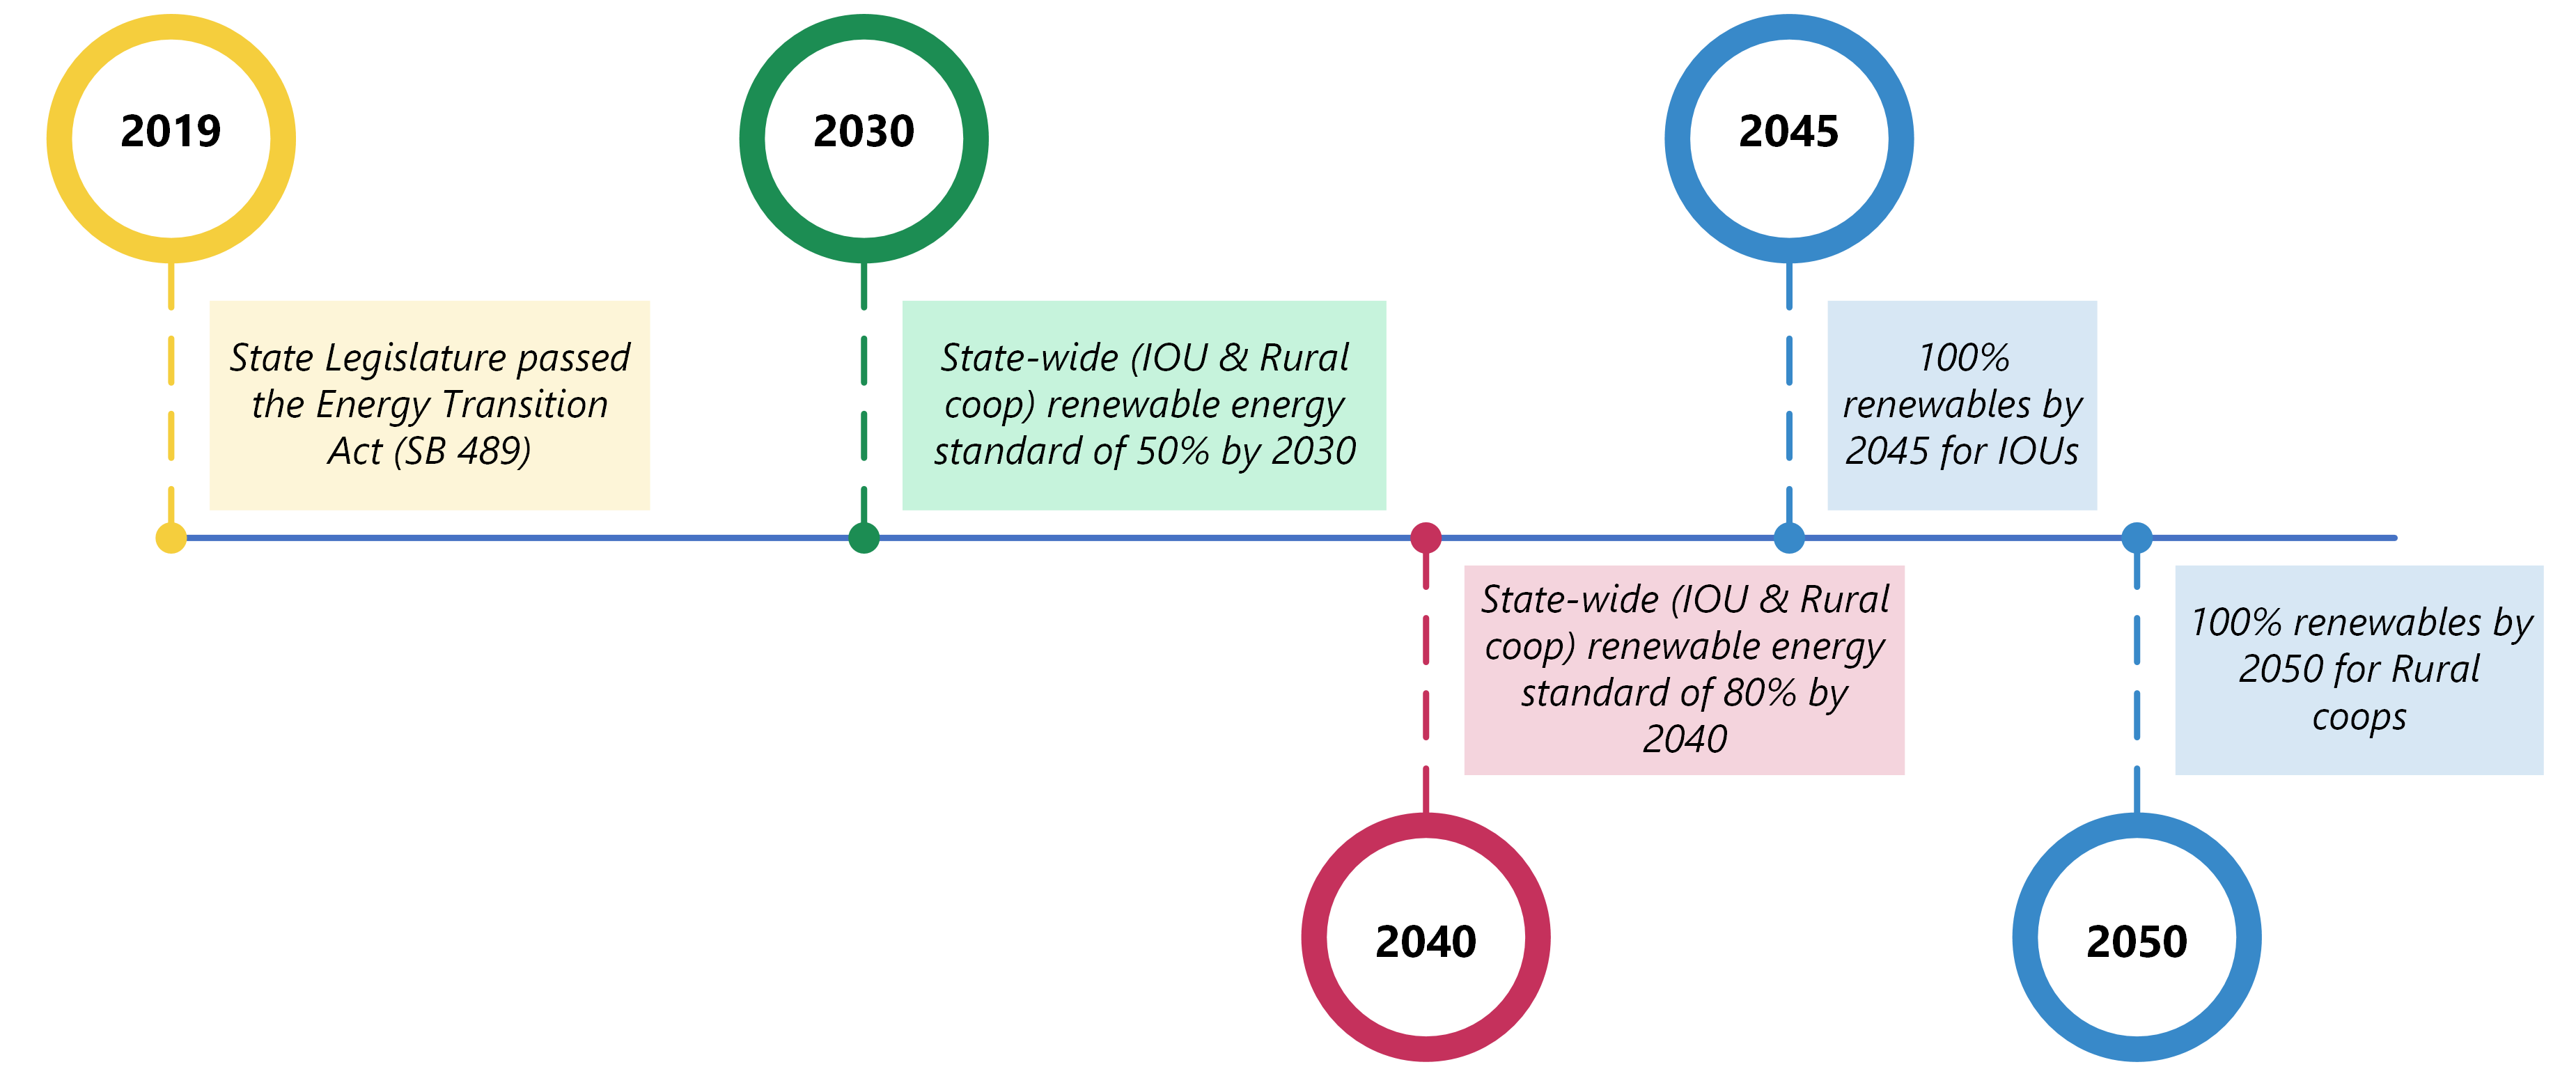
\includegraphics[width=1\textwidth]{figures/nm_eta.png}
    \caption{Timeline of the Energy Transition Act (Senate Bill 489)}
    \label{fig:nm_eta}
\end{figure}

NM is notable for its distinctive demographic composition and climate. Ranking 5th in land area at 121,590 square miles and 36th in population with 2.1 million residents, NM has one of the lowest population densities in the nation \parencite{uscensus2022}.\footnote{NM is the 46th most densely populated state in the nation \parencite{uscensus2022}.} NM is also a majority-minority state, with over 50\% of the population identifies as Hispanic and 11.2\% as Native American \parencite{uscensus2020}.  Around 86\% of the population lives in disadvantaged census tracts defined as overburdened and under-served by the Climate and Economic Justice Screening Tool.\footnote{Author's calculation. See \url{https://screeningtool.geoplatform.gov/en/methodology} for a detailed definition of disadvantaged census tracts.} 

In terms of the state's economy, NM Ranks 41st in GDP per capita among the U.S. states.\footnote{Data source: Statista, Real per capita gross domestic product of United States in 2023, by state \url{https://www.statista.com/statistics/248063/per-capita-us-real-gross-domestic-product-gdp-by-state/}.} NM's economy has been significantly reliant on the oil and gas (O\&G) industry since the discovery of the Permian Basin oil fields in the 1920s. The O\&G industry contributes to around 10\% of NM's annual Gross Domestic Product (GDP) and 25\% and 30\% of the state's tax revenue \parencite{eia2023nm, nmlegislative2023}. This dependency on the fossil fuel industry also poses a challenge to the equitable energy transition.

NM is also well-suited to achieve 100\% renewables as NM boasts abundant wind, solar, and geothermal potential. The state's eastern high plains offer significant wind energy opportunities, while NM ranks third in solar energy potential and sixth in geothermal energy potential nationally. In 2022, renewable sources accounted for 42\% of the state's total electricity generation, well on track to achieve the 2030 50\% renewable target \parencite{eia2023energy}.

The interplay between NM's unique demographics, O\&G dependency, and abundant renewable energy resources underlines the importance of exploring equitable energy transition pathways (\autoref{fig:nm_background}). In this research, we focus on solar photovoltaic (PV) and investigate the current state of residential solar PV adoption in NM and its equity implications. 

\begin{figure}[!ht]
    \centering
    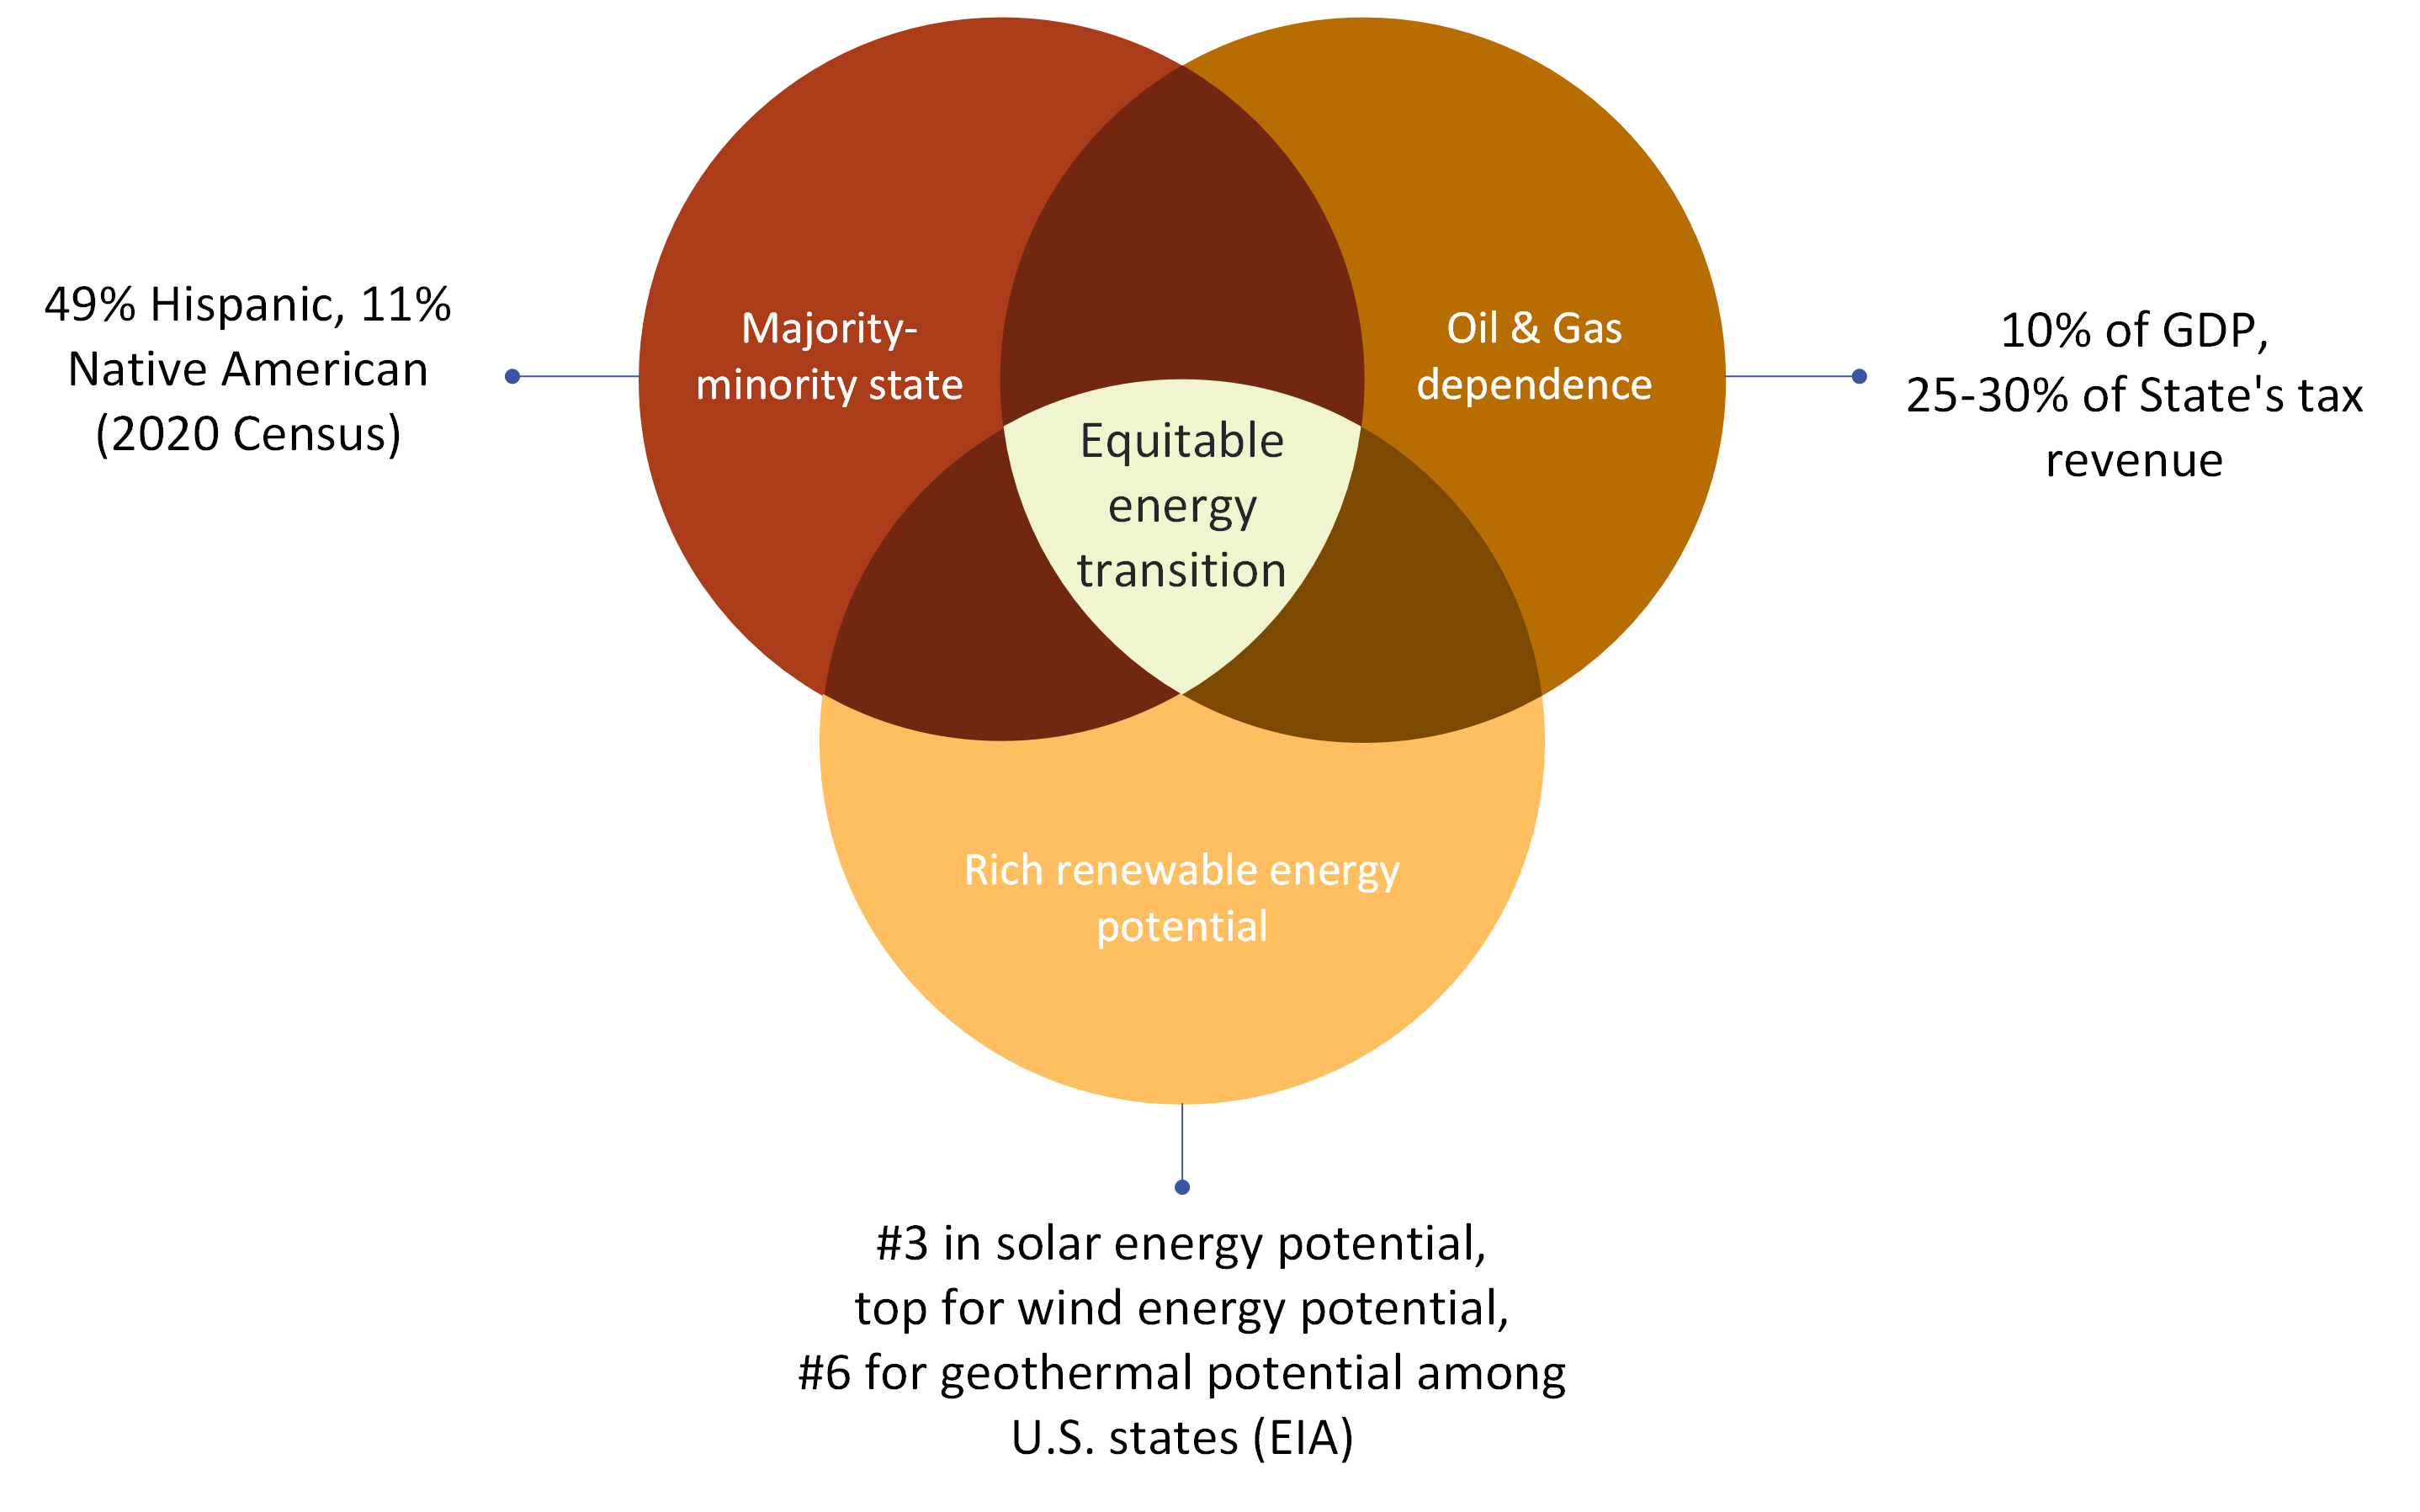
\includegraphics[width=1\textwidth]{figures/nm_background.png}
    \caption{The socioeconomic background of energy transition in New Mexico}
    \label{fig:nm_background}
\end{figure}



\subsection{Equity in energy transition}
\label{section:equity}

In the context of energy transition, the definition of equity encompasses multiple dimensions. The literature can be categorized into three main aspects of equity, namely \textit{access equity}, \textit{adoption equity}, and \textit{distributional equity}. In the following, we review the literature on equitable energy transition with a particular focus on residential solar PV. We also explain the relevance of considering the different aspects of equity in the NM context.

\subsubsection{Access equity}

 Access equity refers to the availability and accessibility of clean energy technologies for all communities, regardless of income, race, or geographic location. \textcite{brockway_inequitable_2021} find using California data that existing grid infrastructure may not be sufficiently robust to handle the increased load from widespread solar PV installations without significant upgrades. This can lead to inequitable access, where certain regions or communities might have lesser ability to connect their solar systems to the grid due to these capacity issues. This finding is relevant in the NM context as solar installations are concentrated in urban areas where in some areas grid infrastructure limits solar installations. For example, in parts of Albuquerque and Rio Rancho, the feeder grids are already at maximum capacity.\footnote{See \url{https://pnm.maps.arcgis.com/apps/webappviewer/index.html?id=cbd3bad85fc64f2180dda652e957bacd} for areas with maximum feeder capacity.} Residents in those communities cannot be approved for new solar installations with grid interconnection until the infrastructure is upgraded.\footnote{In 2021, 2022, and 2023, the Public Service Company of New Mexico (PNM) put 96, 70, and 29 new solar applications on hold, respectively, due to a lack of feeder capacity \parencite{pnm2021,pnm2022,pnm2023}. }

 In addition to grid constraints, other technical barriers, including the lack of suitable roof space or home ownership, or financial barriers, such as high upfront cost, can also limit the ability of some households to adopt solar PV.
 
 \subsubsection{Adoption equity}

 Adoption equity refers to the equitable adoption of solar PV across different socio-economic groups, in particular, income groups and racial and ethnic groups. Researchers have identified several factors that lead to inequitable adoption, including racial and ethnic disparities, income disparities, education level, and renter-owner status \parencite{gao_solar_2022, darghouth_characterizing_2022, lukanov_distributed_2019, best_meta-analysis_2023}. For example, \textcite{gao_solar_2022} find that while racial and ethnic disparities in solar PV adoption have decreased from 2012 to 2019, households in Asian-, Black-, and Hispanic-majority census tracts still install fewer systems compared to White-majority tracts. \textcite{darghouth_characterizing_2022} find significant income inequality in U.S. rooftop solar adoption, with higher-income households more likely to install solar PV systems. They also identify greater solar adoption equity in areas with higher racial diversity, higher levels of education, and higher owner-occupancy rates, as well as among census tracts served by smaller and low- and moderate-income (LMI)-focused installers. However, \textcite{reames_exploring_2021} finds that while communities of color have slightly lower rooftop solar potential than majority-white areas, the disparities are not significant enough to justify the large differences in solar adoption rates. These insights highlight the need for policies that address racial equity, income, and home-ownership status in the clean energy transition. \textcite{oshaughnessy_income-targeted_2021}  highlight the role of supply-side barriers in solar equity by revealing that solar installers submit fewer quotes to low-income households, significantly reducing their likelihood of adopting solar panels.

 The literature has also examined the effectiveness of various policies to improve equity in solar adoption. \textcite{gao_solar_2022} find local and utility-level solar justice policies that aim to promote solar PV adoption by broader and more diverse segments of populations in the U.S. positively impact low-income households’ adoption rates, but these policies are less effective in Black-majority census tracts, indicating that non-financial barriers also need to be addressed. \textcite{darghouth_characterizing_2022} find falling solar PV costs reduce the impact of price on adoption inequity, suggesting that policy interventions should focus on structural barriers and supporting diverse installer practices. \textcite{oshaughnessy_rooftop_2022} concludes that financial incentives like grants, rebates, and tax credits are highly effective in promoting and sustaining solar adoption among LMI households. \textcite{oshaughnessy_impact_2021} find that in addition to tax credits, rebates, and direct subsidies, innovative business models like solar leasing significantly enhance solar adoption among LMI households. 

    Examining the issue of adoption equity is particularly relevant in NM given its high share of minority and disadvantaged populations and significant variance in income and education levels. NM also implements generous solar incentives, such as state solar tax credits and utility net energy metering (NEM) policies. Therefore, it is important to evaluate whether these policies alleviate or exacerbate adoption equity in the NM context.

\subsubsection{Distributional equity}

Distributional equity refers to whether the benefits of clean energy incentives are uniformly distributed across different demographic groups. The issue of distributional inequality is not limited to incentives for solar adoption. \textcite{borenstein_distributional_2016} use tax filing data to examine the uptake of four major clean energy tax credits: weatherization (Nonbusiness Energy Property Credit), residential solar (Residential Energy Efficient Property Credit), hybrid and electric vehicles (Alternative Motor Vehicle Credit), and plug-in electric vehicles (Qualified Plug-In Electric Drive Motor Vehicle Credit). They find significant inequities in the distribution of tax credits, with the top income quintile receiving about 60\% of all clean energy tax credits, while the bottom three income quintiles receive about 10\%. \textcite{jacobsen_race_2024} uses survey data from the Residential Energy Consumption Survey (RECS) and finds significant racial and ethnic disparities in the receipt of energy efficiency incentives in the U.S., driven primarily by differences in home-ownership rates. As NM provides state solar tax credits to households, understanding the distributional effect of existing credits provides insights into efficient and equitable policy design.

\subsection[Policy background]{Policy background}

Incentives to promote solar PV adoption in the residential sector have been implemented at different regulatory levels, from federal to service-providing utilities. These incentives play important roles in the households' decision-making of going solar. All incentives are essentially financial, which either lowers the upfront cost of solar investment or reduces the payback period of solar. In the remainder of this section, we review the incentives available to NM households since 2005 for solar PV investments. \autoref{fig:nm_incentive} summarizes the various incentives and their respective policy time spans. For each incentive, we describe the incentive structure, time of initiation and expiration, and eligibility. 

\begin{figure}[H]
    \centering
    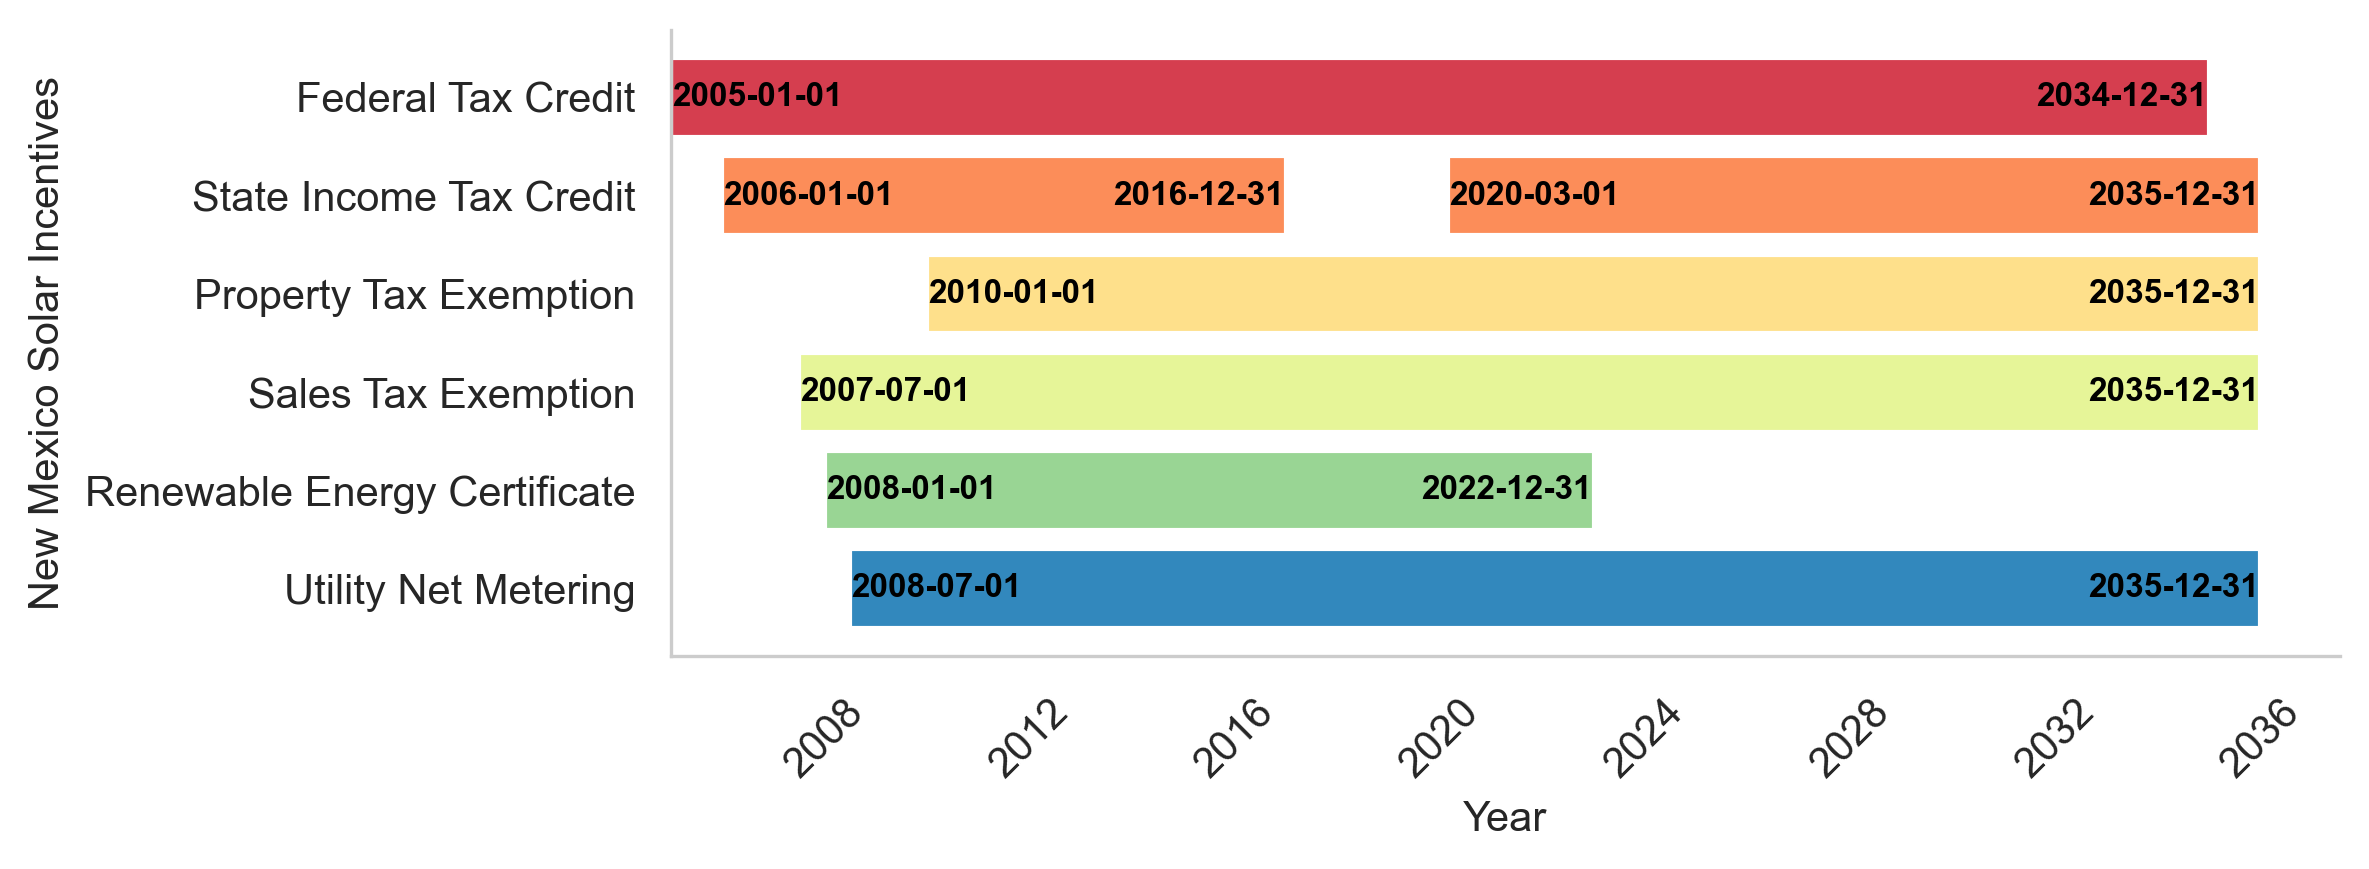
\includegraphics[width=1\textwidth]{figures/policy_timeline.png}
    \caption{Incentives for residential solar PV in New Mexico}
    \label{fig:nm_incentive}
    \begin{flushleft}
        \footnotesize Note: For policies with no definitive end dates, the end date is not displayed in the timeline.
    \end{flushleft}
\end{figure}

\subsubsection{Federal incentives}


The federal tax credit for solar panel installations, also known as the Investment Tax Credit (ITC), was initially introduced in the Energy Policy Act in 2005. It provided a tax credit of 30\% for residential and commercial solar energy installations. ITC was extended multiple times and maintained a 30\% credit for solar installations through 2019. The tax credit percentage was stepped down in 2020, where the systems installed in 2020 and 2021 were eligible for a 26\% tax credit \parencite{doeitc}. ITC was originally set to phase down after 2022 (26\% in 2022, 22\% in 2023, 0\% by 2024) before the introduction of the Inflation Reduction Act (IRA) in 2022. IRA extended the ITC, now known as the Residential Clean Energy Credit, which provides a 30\% tax credit from 2022 through 2032. The credit rate phases down to 26\% in 2033 and 22\% in 2034, unless otherwise noted. The federal tax credit places no limit on the total amount claimed, and any credit exceeding tax liability can be carried forward to future tax years \parencite{irs}.

\subsubsection{State incentives}

\textbf{Solar tax credit}

Since the 2000s, the importance of renewable energy in reducing greenhouse gas emissions and combating climate change has been increasingly recognized. In response, NM initiated a solar tax credit in 2006, known as the Solar Market Development Tax Credit (SMDTC). The SMDTC was effective from January 1, 2006, through December 31, 2016, and offered 10\% tax credit on the total installation costs of solar panel systems, with a maximum credit amount of \$9,000 per taxpayer per taxable year. The SMDTC was reinstated in 2020, known as the New Solar Market Development Tax Credit (NSMDTC). Solar PV systems installed after March 1, 2020 are eligible for a 10\% tax credit on the total installation costs with a maximum credit amount of \$6,000. The total tax credit issued within the state is capped at 8 million dollars for the tax years 2020  and 2021, and 12 million dollars since 2022.\footnote{In 2021, 2022, and 2023, the credit cap was reached. \url{https://nm-emnrd.maps.arcgis.com/apps/dashboards/e882d2ccd57e4a99bc6d2a4314fcd3bb}} There is no income threshold to claim the tax and all credit exceeding the taxpayers' liability are refunded instead of carrying over to subsequent tax years \parencite{nmsmdtc}. 

\noindent\textbf{Property tax exemption}

Under House Bill 233, enacted by the NM legislature in 2010, residential solar systems are not treated as physical improvements and therefore do not increase the value of the property for property tax purposes. However, future assessments can include the value of a solar energy system if the property is sold \parencite{propertytax}. This exemption provides a financial incentive for homeowners since installing solar PV increases property value on the housing market without incurring additional property taxes.


\noindent\textbf{Sales tax exemption}

The NM Gross Receipts Tax Exemption policy for solar energy systems, effective since 2007, allows businesses to deduct receipts from selling solar equipment or installation services \parencite{NMStat2021}. Essentially, for consumers, there is no sales tax on top of the cost of solar installation, which reduces the financial burden on solar adopters.


\noindent\textbf{Renewable energy certificates}

The New Mexico Renewable Energy Certificate (REC) policy for solar PV is part of the state's broader Renewable Portfolio Standard (RPS). The RPS requires that IOUs must secure 50\% of their capacity through carbon-free renewables by 2030 and 100\% by 2045. For rural electric cooperatives, the goals are 40\% by 2025, 50\% by 2030, and 100\% by 2050. The IOUs in NM thus offered Renewable Energy Certificate (REC) purchase agreements to solar owners for a limited time to count residential solar generation toward their required RPS. The Public Service Company of New Mexico (PNM) offered a Solar Renewable Energy Certificate (SREC) program that awards systems a stepped purchased rate for the energy generated for residential systems. This program was discontinued at the end of 2022 \parencite{pnmrec}. The El Paso Electric Company (EPE) offered a tiered REC purchase rate for systems installed before 2017, which ended on December 31, 2020 \parencite{eperec, eperecmid}.\footnote{Details on the purchase agreements can be found on the respective company's websites.}

\subsubsection{Utility incentives}

Utility companies in NM, including IOUs, rural cooperatives, and public utilities, are mandated by the NM Public Regulatory Commission (NM PRC) to offer net energy metering (NEM) programs to solar customers. Under NEM, solar customers who generate excess electricity with their solar panel systems can send it back to the grid and receive credits. These credits can be used to offset future electricity use.\footnote{For example, if the solar panels generate more electricity during the day than the household consumes, the excess electricity is sent back to the grid, and the meter runs backward, creating a credit. At night, when solar panels do not produce electricity, the household consumes electricity from the grid and the meter runs forward.} However, the details of the NEM program vary by utility. For example, PNM offers a net metering program for all residential solar systems. For small PV systems (inverter capacity lower than 10 kW-AC), any excess generation for the month (when monthly usage is lower than total monthly generation) is credited to the customer’s account and can be used for future billing cycles, never expiring unless the account is closed. Excess generation from large PV systems (inverter capacity greater than 10 kW-AC) is paid each month at the predetermined energy purchase rate for that month \parencite{pnmnet}. El Paso Electric (EPE) offers net metering for all systems within a billing cycle, but all excess generation for the month is paid out to customers at the predetermined purchase rate \parencite{epenet, epenetmid}. The purchase rate for the credits is typically lower than the retail electricity price for all utilities.\footnote{For example, in 2023, the PNM power purchase rate ranged from 3 to 12 cents per kWh, depending on the month, while the retail rate was 7.8 cents per kWh for the first 450 kWh per month, increasing to 15 cents per kWh thereafter.} The differences in NEM incentives provide a quasi-experimental setting to study how NEM policy design incentivizes residential solar adoption. 

%%%%%%%%%%%%%%%%%%%%%%%%%%%%%%%%%%%%
% \section{Current trend  and distribution of residential solar in New Mexico}
\customsection{Current trend  and distribution}{Current trend  and distribution of residential solar in New Mexico} %header shows the name in first braces

In this section, we utilize detailed solar installation data collected from state agencies and utilities to illustrate the trends and distribution of solar installations in NM. Our focus is on the distribution across geographical areas, income groups, and racial and ethnic groups for both installation counts and system capacities.

\subsection{Data description}
\label{section:data_collect}

To provide a comprehensive overview of solar installations in NM, we assembled a unique dataset from various public and restricted sources. This dataset includes system-level characteristics, housing characteristics, census tract-level demographics, and spatial data on climate and community types. The following sections detail the dataset components.

\subsubsection{Installation data}

We obtain system-level solar installation data from three sources: the New Mexico Energy, Minerals, Natural Resources Department (EMNRD), and the New Mexico Public Regulatory Commission (NMPRC) document archive eDocket database, and individual utilities. 

EMNRD oversees solar tax credit claims under the SMDTC and NSMDTC programs. Their data includes all systems that were approved for the state tax credits between the programs' active periods (2006-2016 and 2020 onwards). This data, acquired through a non-disclosure agreement, includes identifying information about solar households. It provides details on the installation location, grid connection date, system size, installer name, system cost, and approved state credit amount, encompassing 20,159 unique residential systems.

The NMPRC eDocket database contains records of annual compliance filings by state-regulated utilities (IOUs and rural cooperatives) under Rule 17.9.570.13(G) NMAC.\footnote{Details of Rule 17.9.570 can be found here: \url{https://www.srca.nm.gov/parts/title17/17.009.0570.html}.} This rule mandates utilities to report the name and location of interconnected solar systems, annual purchases from these systems, and any rejected interconnection applications. Due to varying data quality, we obtain data of the two largest IOUs in the state, PNM and EPE, and one rural cooperative, Socorro Electric Coop (SEC). Together, they account for over 90\% of solar customers in NM, providing data on system location, interconnection date, and installed capacity for 50,416 residential systems.

Public utilities, not subject to NMPRC rulings, provided solar system data directly. We obtain data from the Los Alamos Department of Public Utilities (LADPU) for the 427 residential solar systems in their service area.


\subsubsection{Housing characteristics data}

We scrap housing characteristics data from Zillow using the addresses in the installation data. This data includes variables such as year built, number of bedrooms and bathrooms, estimated home value (Zestimate), living area size, lot size, parking features, heating and cooling technologies, and geographic coordinates.\footnote{NM is a non-disclosure state, meaning the actual transaction price of homes is not public information.} Housing information was available for 65,125 systems in the combined installation dataset.

\subsubsection{Census tract-level demographics data}

Using the geographical information from the housing data (longitude and latitude), each system was placed in a census tract using the Census Bureau’s tract shape file. We gathered census tract-level demographic variables from the 2010 and 2020 Decennial Census and the American Community Survey from 2010 to 2022. The demographic data includes the following variable categories: 1) housing characteristics (total housing units, occupancy rate, owner occupancy rate, average number of rooms and housing size, main energy source, mortgage rate, housing value, and age of housing); 2) racial composition (racial diversity, percentages of white, Native American, and Hispanic populations); and 3) other demographics (percentage of male population, age distribution, education level, total population, area median income, and urban/rural classification).

\subsubsection{Other relevant data}

Additionally, we complemented the main dataset with average annual electricity prices by utility from the Energy Information Administration (EIA) \parencite{eiaprice}, spatial weather data from Solargis, including Global Horizontal Irradiation (GHI) and average annual temperature \parencite{solargis}, and the community disadvantage status from the Climate and Economic Justice Screening
Tool \parencite{cejst}.

In summary, our comprehensive dataset contains 54,462 unique solar installations (full sample) in NM, 49,993 of which have detailed geographical information (restricted sample). We use the full sample in the subsequent analysis when geographical information is not required and use the restricted sample when spatial analysis is needed.

\subsection{Installation time trend}
 
NM has experienced exponential growth in residential solar installations since 2000. As shown in \autoref{fig:culmulative_capacity}, the total installation capacity in 2023 (280 MW) almost doubled that in 2020 (141 MW). By 2023, residential solar accounted for 14.8\% of the state’s total solar capacity \parencite{seia2023nm}.

\begin{figure}[!ht]
    \centering
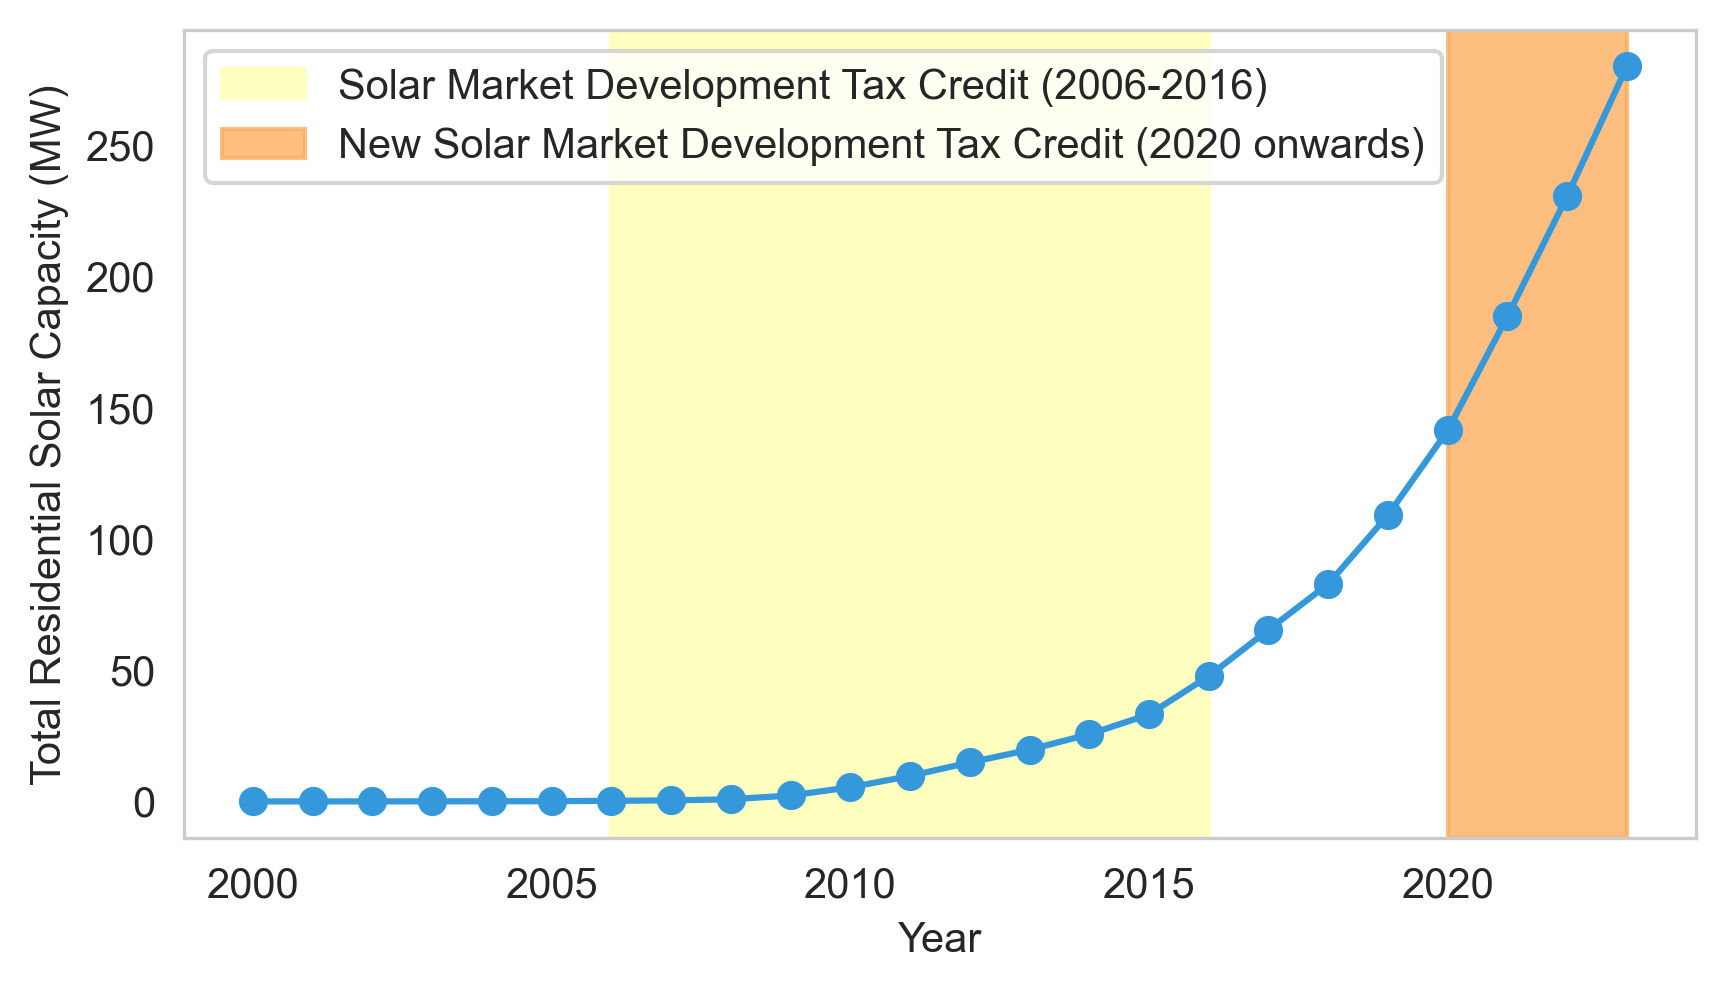
\includegraphics[width=0.9\textwidth]{figures/cumulative_capacity.png}
    \caption{Cumulative residential solar capacity from 2000 to 2023}
    \label{fig:culmulative_capacity}
    \begin{flushleft}
        \footnotesize Note: The line chart shows the cumulative residential solar capacity since 2000 in megawatt (MW). The shaded areas illustrate the policy period of the first and second state solar tax credits.  
    \end{flushleft}
    
\end{figure}


The rapid growth in residential solar can partially be attributed to the significant reduction in the cost of solar panels. \autoref{fig:installation_count} shows the annual installation count in relation to the unit price of the installation. The installation price per kilowatt (kW) of solar PV capacity in 2023 is less than one-third of the price in 2007, making solar an affordable energy source for many households.

State solar tax credits, combined with federal and other incentives, have also facilitated the growing adoption of solar. Figures \ref{fig:culmulative_capacity} and \ref{fig:installation_count} show that in years with tax credits, the adoption level is high, especially when unit prices are lower.

\begin{figure}[H]
    \centering
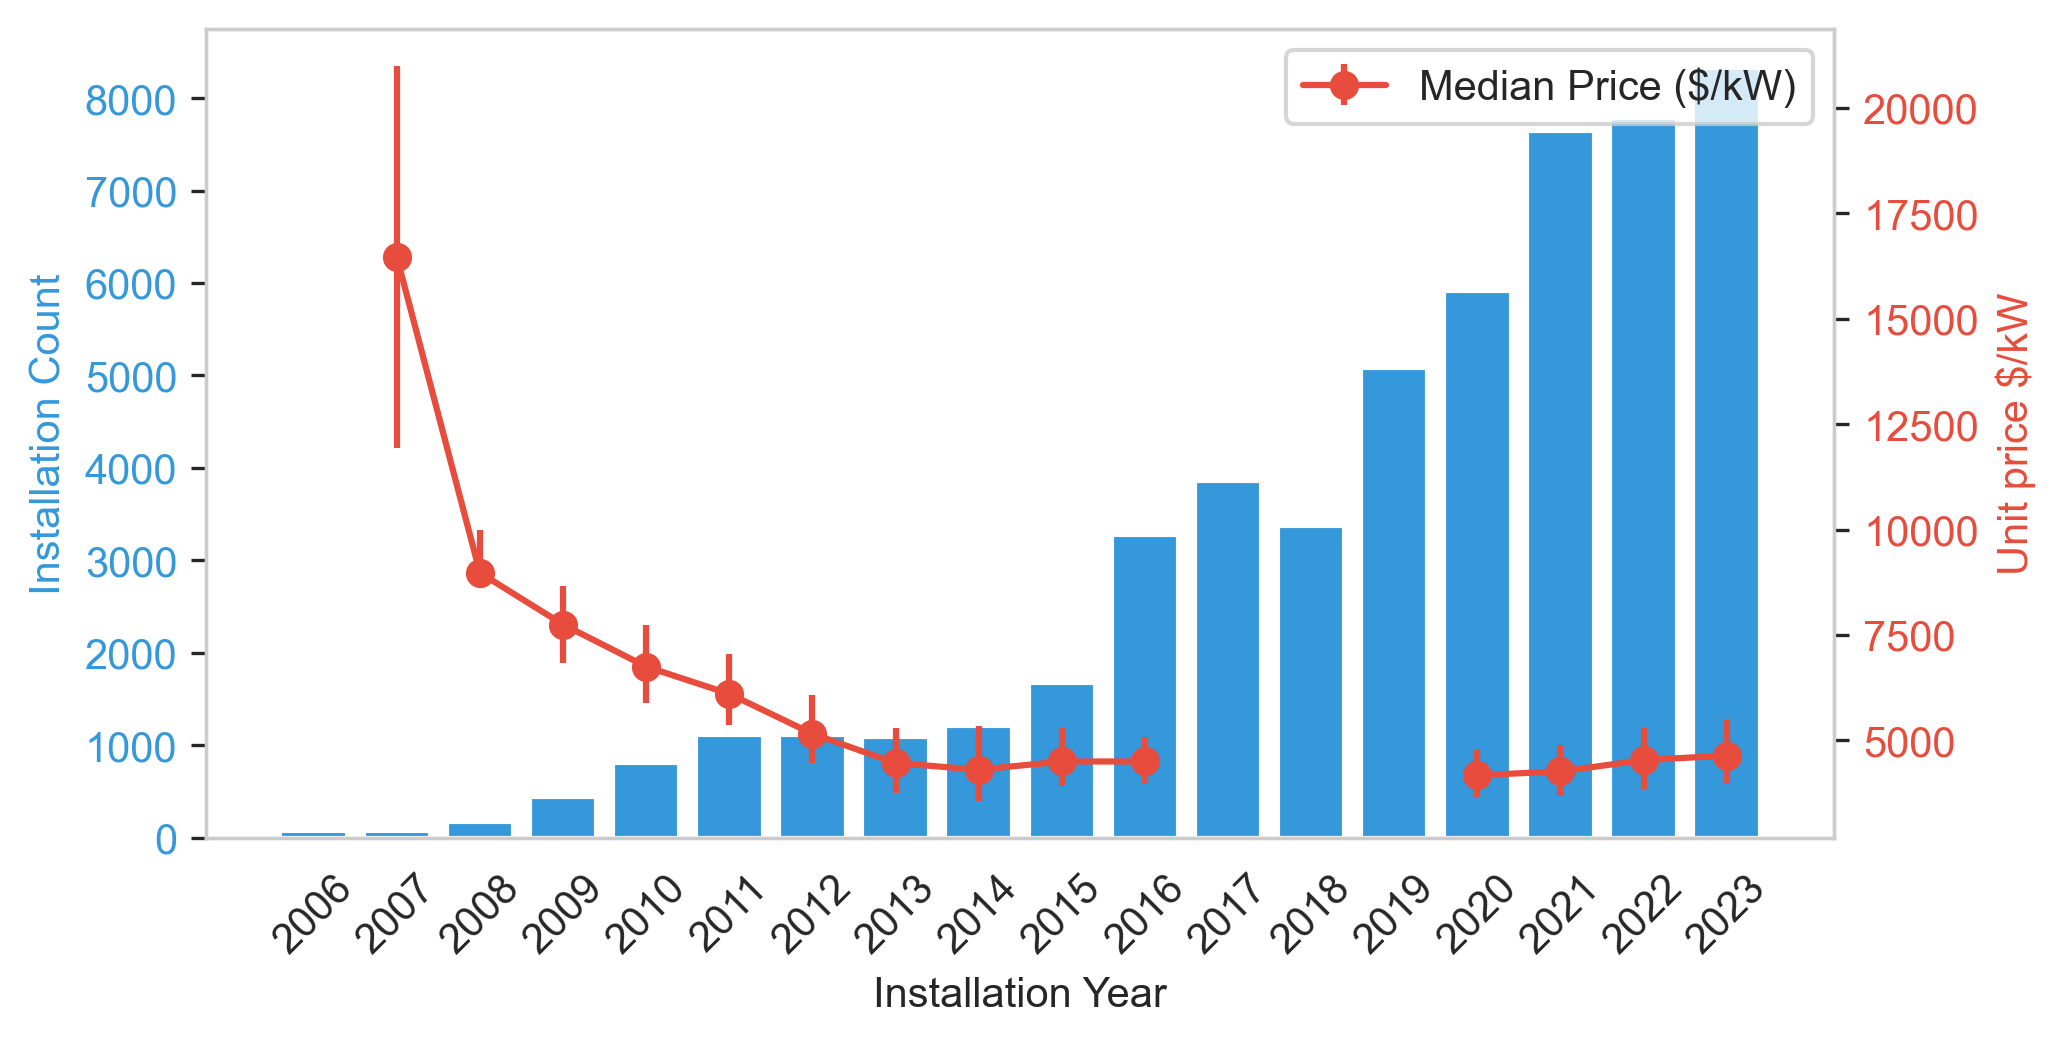
\includegraphics[width=1\textwidth]{figures/installation_count_price.png}
    \caption{Annual solar installation count and unit price in New Mexico}
    \label{fig:installation_count}
    \begin{flushleft}
        \footnotesize The error bars show the 25\% to 75\% range of the unit prices (\$/kW). The installed price ranges exclude any systems with battery storage. In the years 2017 to 2019, the state’s solar tax credit program was not available. Therefore, price information is missing for those years.
    \end{flushleft}
\end{figure}

\subsection{Distribution of solar installation}

\subsubsection{Spatial distribution}

The growth in solar adoption is not uniformly distributed across NM. \autoref{fig:tract_map} shows the total installations by census tract. It is evident that current solar installations are concentrated in the most populous cities of NM, namely Albuquerque, Santa Fe, and Las Cruces. Even after adjusting for population density (\autoref{fig:install_kpop}), there is still a higher installation per thousand people in these cities, indicating an urban/rural disparity in solar adoption.

\begin{figure}[H]
    \centering
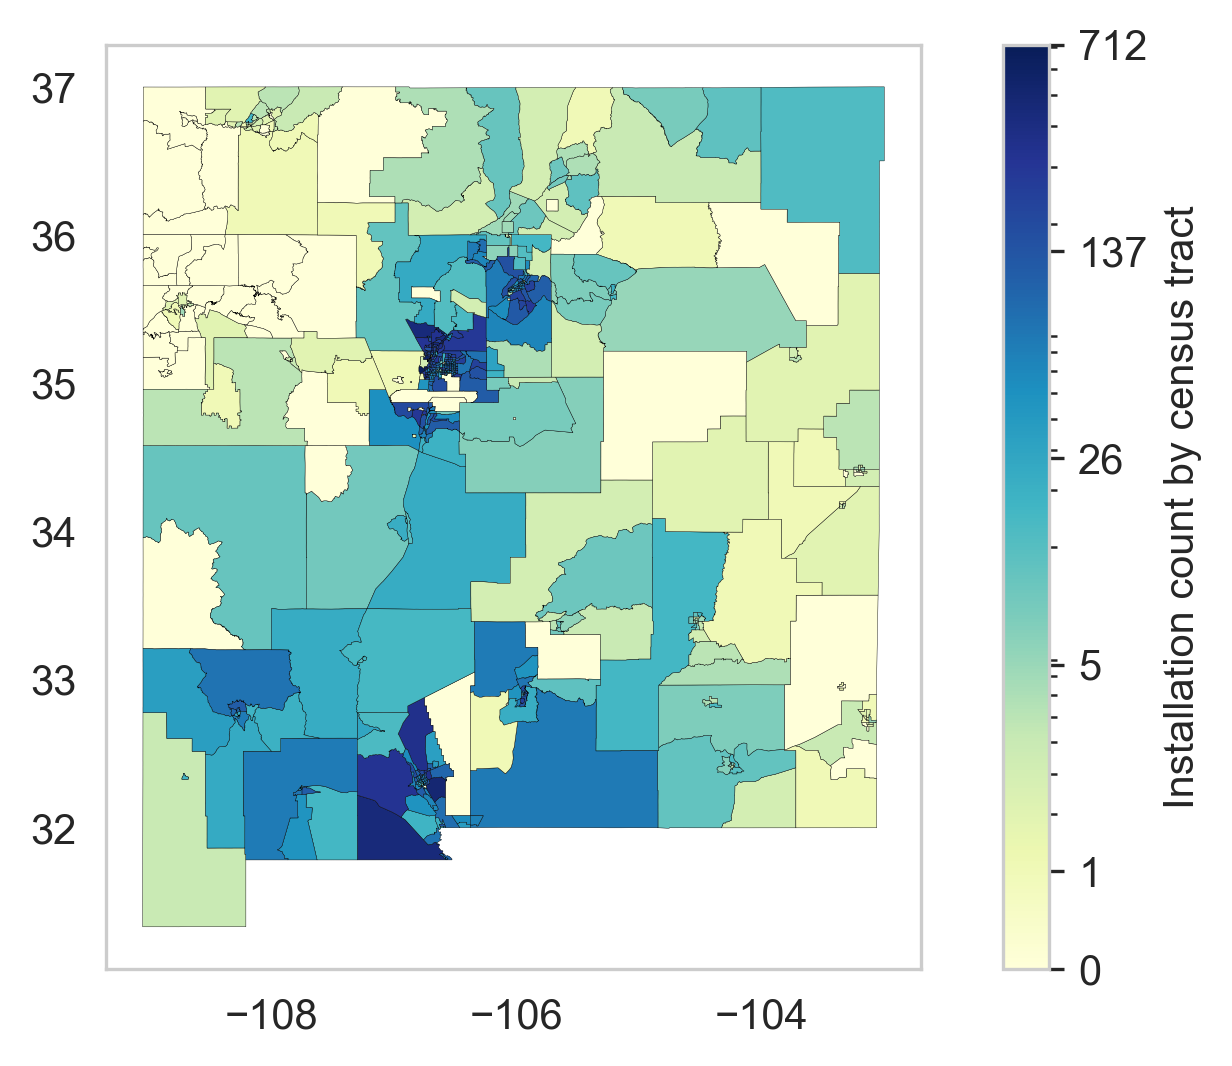
\includegraphics[width=0.7\textwidth]{figures/tract_count_map.png}
    \caption{Total installation count by census tract}
    \label{fig:tract_map}
    \begin{flushleft}
        \footnotesize Note: The total installation count is up to the end of 2023 for each census tract. The census tracts are defined in the 2020 Decennial Census. The legend is in logarithmic scale.
    \end{flushleft}
\end{figure}

\autoref{fig:disadvantage_installation} illustrates the distribution of installations with respect to disadvantaged census tracts within NM. Disadvantaged census tracts are defined as “census tracts that are overburdened and underserved” by the Justice40 Initiative \parencite{justice40}. While 86\% of the population in NM lives in disadvantaged communities, less than 29\% of the solar installations are within those communities (orange dots in the figure).

\begin{figure}[H]
    \centering
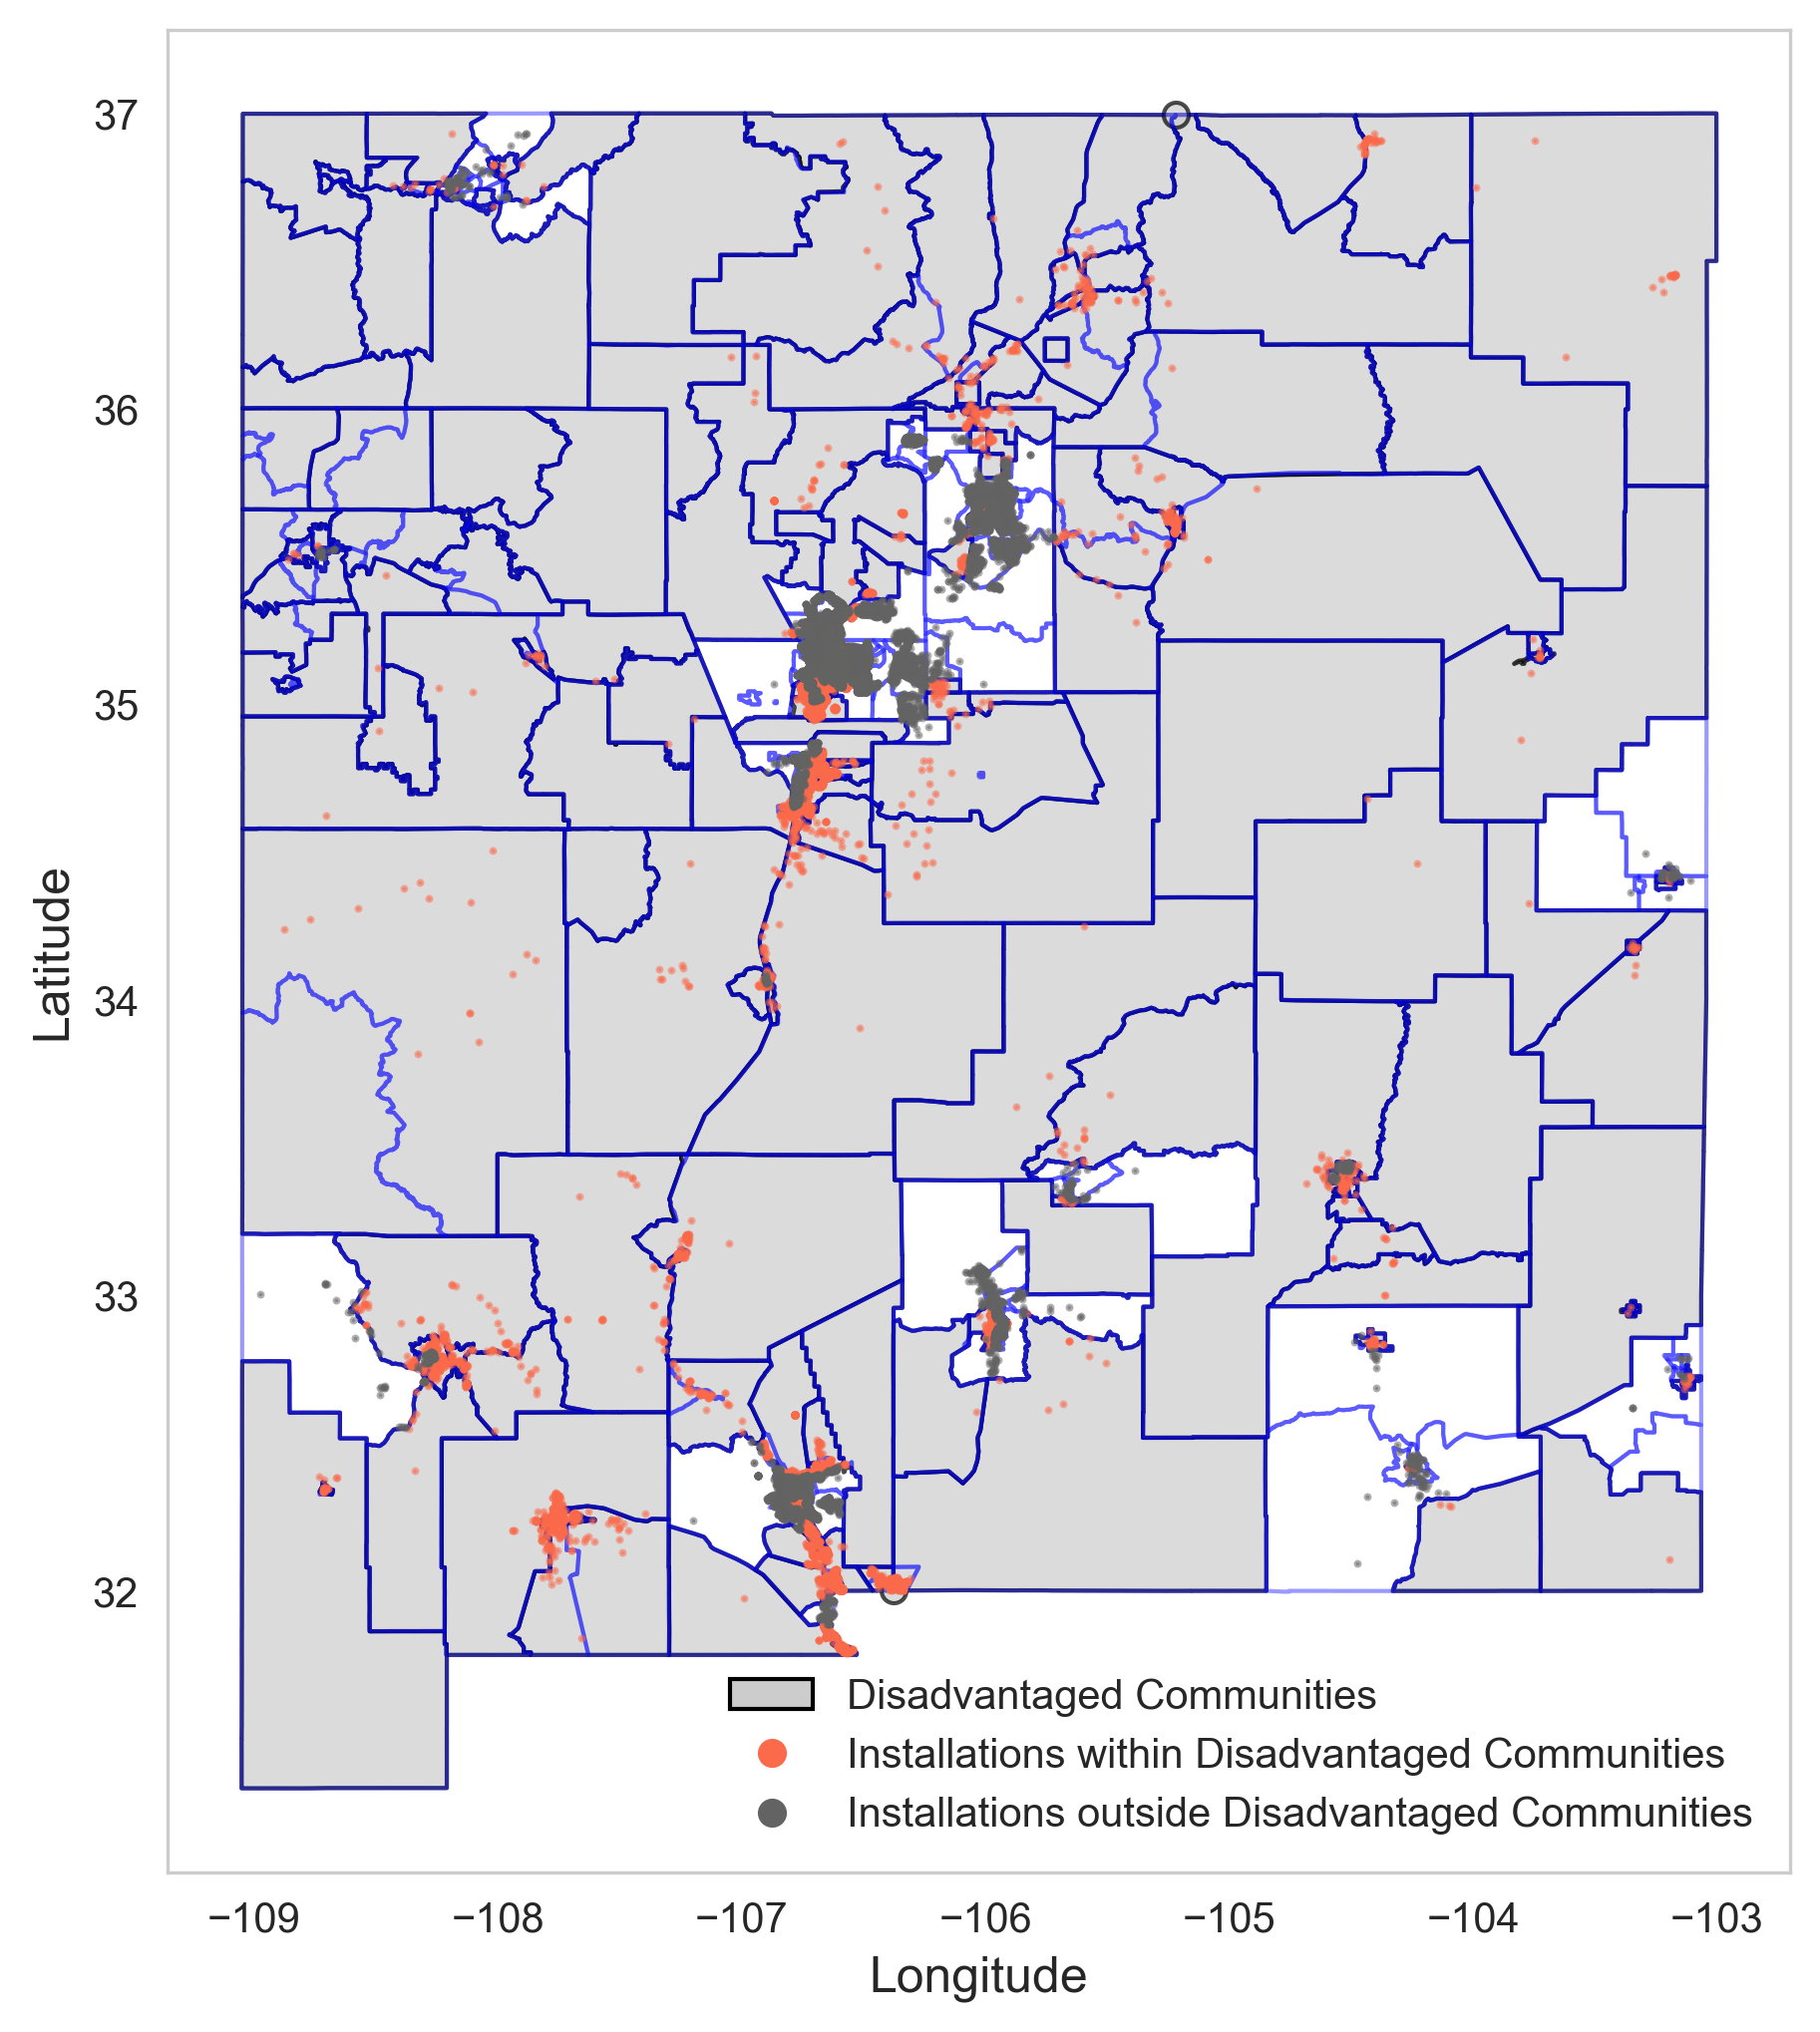
\includegraphics[width=0.7\textwidth]{figures/disadvantage_installation.png}
    \caption{Installation within and outside disadvantaged communities}
    \label{fig:disadvantage_installation}
        \begin{flushleft}
        \footnotesize Note: Disadvantage communities shape file retrieved from the Climate and Economic Justice Screening Tool \url{https://screeningtool.geoplatform.gov/en/#10.84/36.2534/-104.868}. Census tracts that are overburdened and underserved are highlighted as being disadvantaged on the map.
    \end{flushleft}
\end{figure}


\subsubsection{Income distribution}

Consistent with existing research, census tracts in NM with higher area median income (AMI) also have more households installing solar, even when adjusted for population. \autoref{fig:population_ami_count} reveals a positive correlation between AMI and installation per thousand population.

\begin{figure}[h]
    \centering
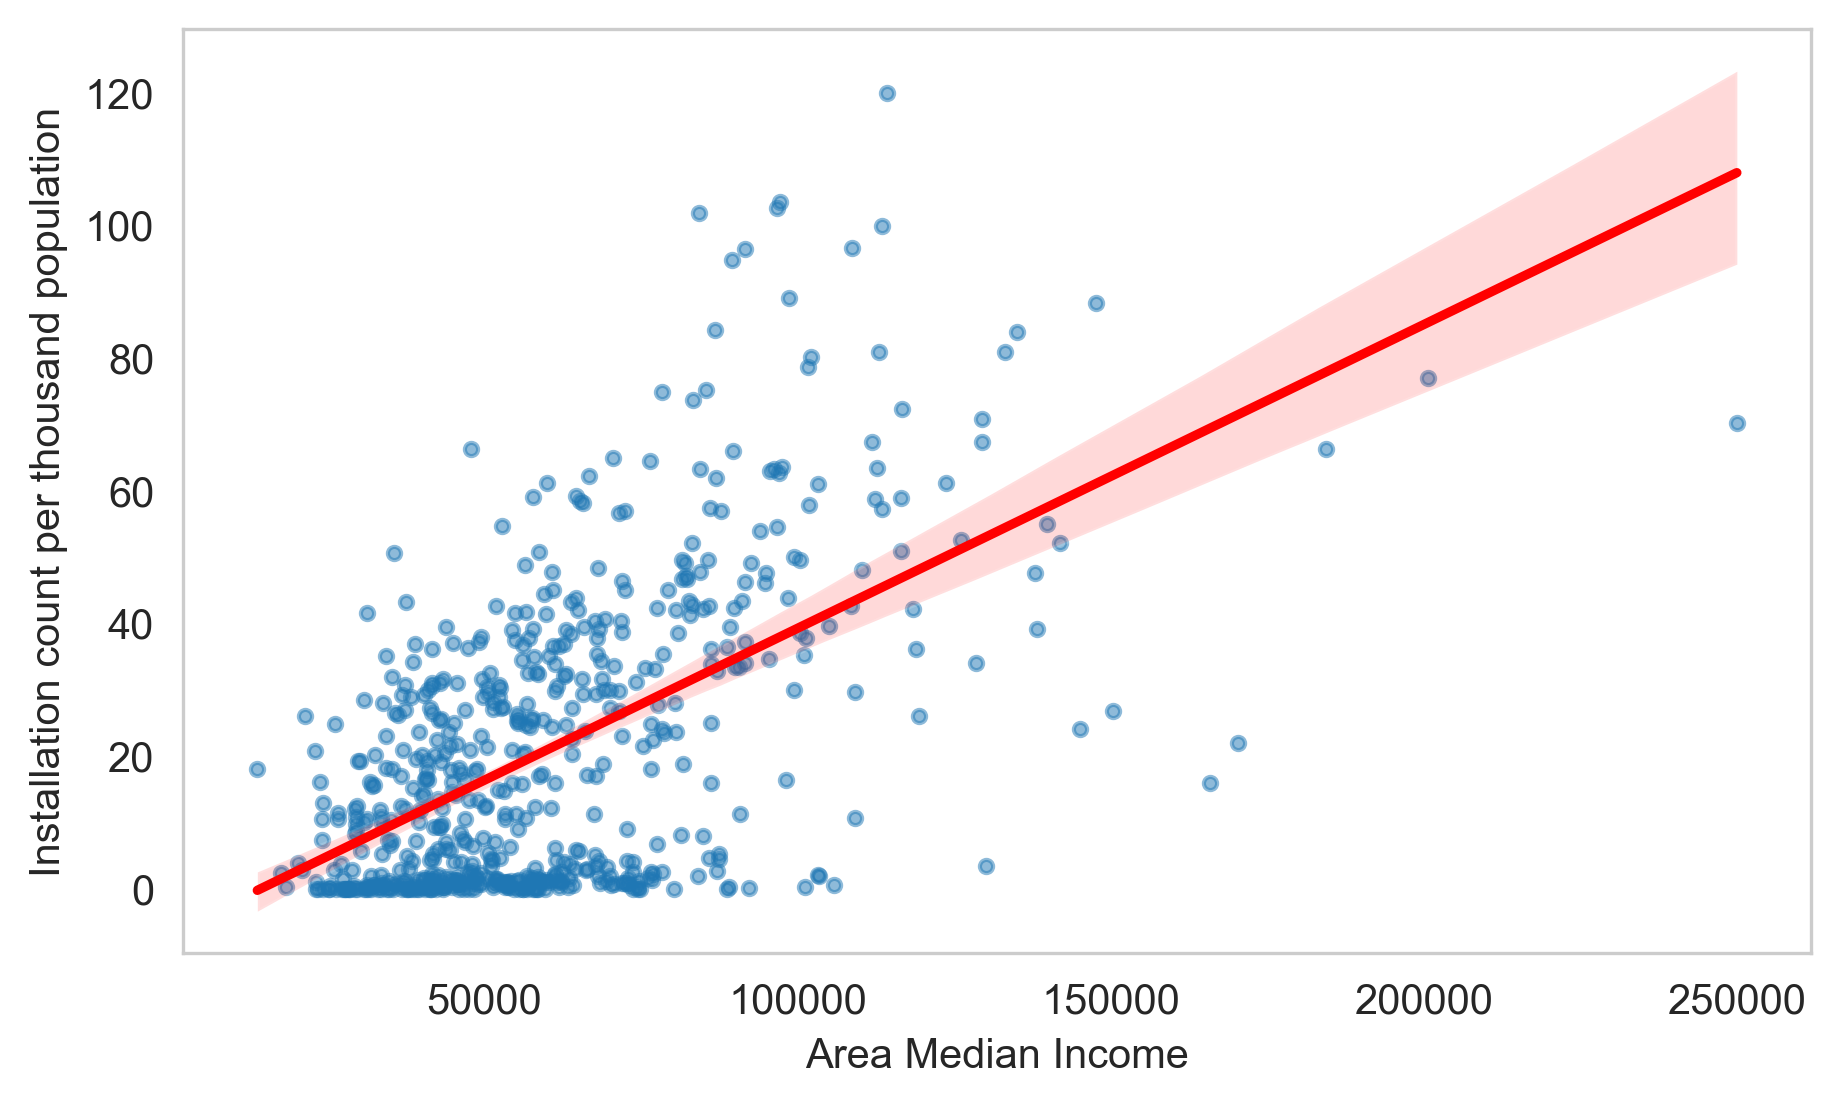
\includegraphics[width=0.9\textwidth]{figures/population_ami_count.png}
    \caption{Installation per thousand population by area median income}
    \label{fig:population_ami_count}
        \begin{flushleft}
        \footnotesize Note: The population and area median income (AMI) are based on 2022 data from the American Community Survey 1-year data. Census tracts with an AMI higher than 250,000 are capped at 250,000. The shaded area around the regression line represents the 95\% confidence interval.
    \end{flushleft}
\end{figure}

\subsubsection{Racial and ethnic distribution}

NM is characterized by a diverse racial and ethnic composition. The majority of the population identifies as White alone, comprising 51\% of the total population \parencite{uscensus2020}. Significant proportions include American Indian and Alaska Native (10\%), Black or African American (2.2\%), Asian (1.8\%), individuals identifying as Some Other Race alone (15.0\%), and those identifying as two or more races (19.9\%). The population is almost evenly split between Hispanic (47.7\%) and non-Hispanic (52.3\%), with 36.5\% being White non-Hispanic.

Out of the 612 census tracts, 64\% are White-majority (defined as more than 50\% of the population identifies as White alone), and 38\% are Hispanic-majority. Examining the total installation count by majority status (\autoref{fig:installation_race}) reveals a significant concentration of installations in White-majority census tracts across all years. The difference between Hispanic and non-Hispanic census tracts is much smaller, with slightly higher installation counts in non-Hispanic tracts. \autoref{fig:population_quintiles} confirms this when breaking down the data into five bins of population shares instead of majority status. 

\begin{figure}[!ht]
    \centering
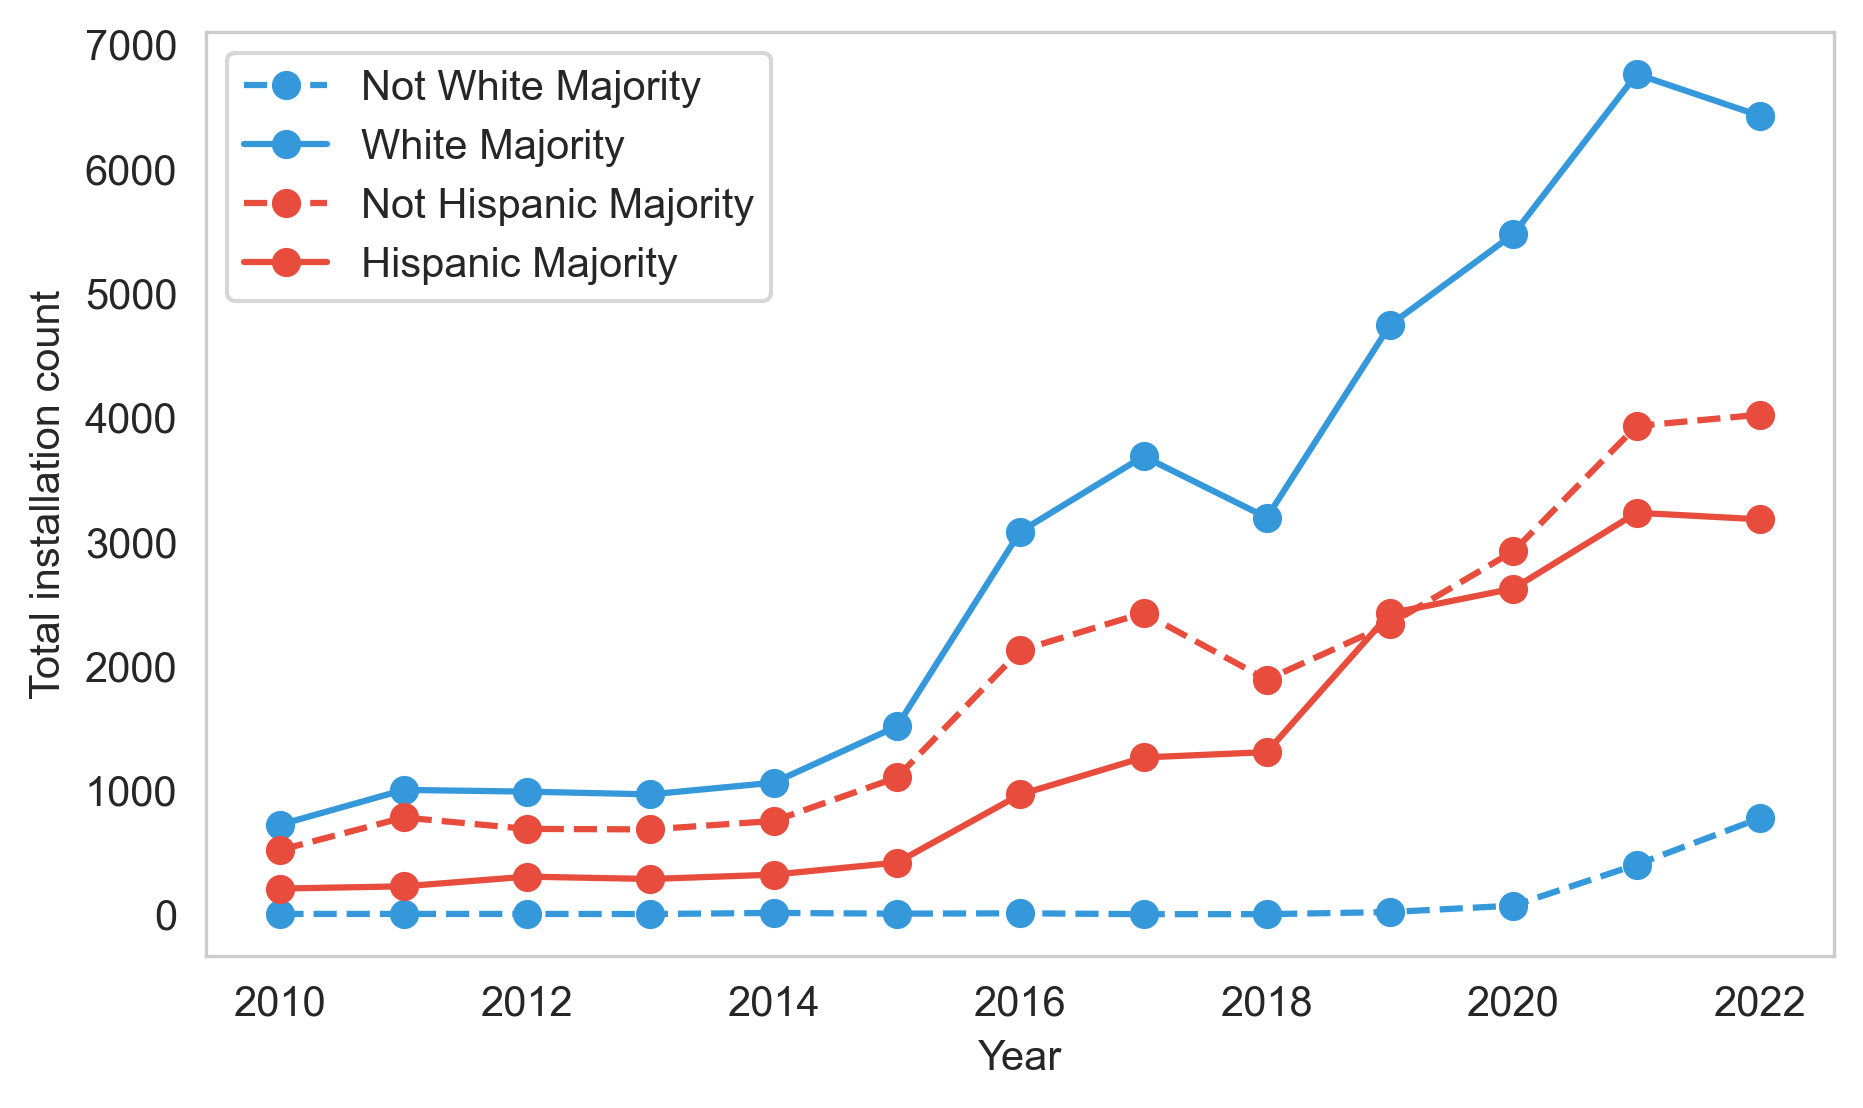
\includegraphics[width=0.9\textwidth]{figures/installation_by_race.png}
    \caption{Annual installation by racial majority group}
    \label{fig:installation_race}
        \begin{flushleft}
        \footnotesize Note: White majority refers to census tracts where more than 50\% of the population identifies as White alone. Hispanic majority refers to census tracts where more than 50\% of the population identifies as Hispanic.
    \end{flushleft}
\end{figure}



\subsubsection{Capacity distribution}

The capacity of installed systems varies among solar households. \autoref{fig:capacity_density} displays the distribution and cumulative distribution function (CDF) of system capacities (in kW). Most system capacities are clustered between 2 kW and 8 kW, with half of the systems below 5 kW and 95\% below 10 kW.


\begin{figure}[!ht]
    \centering
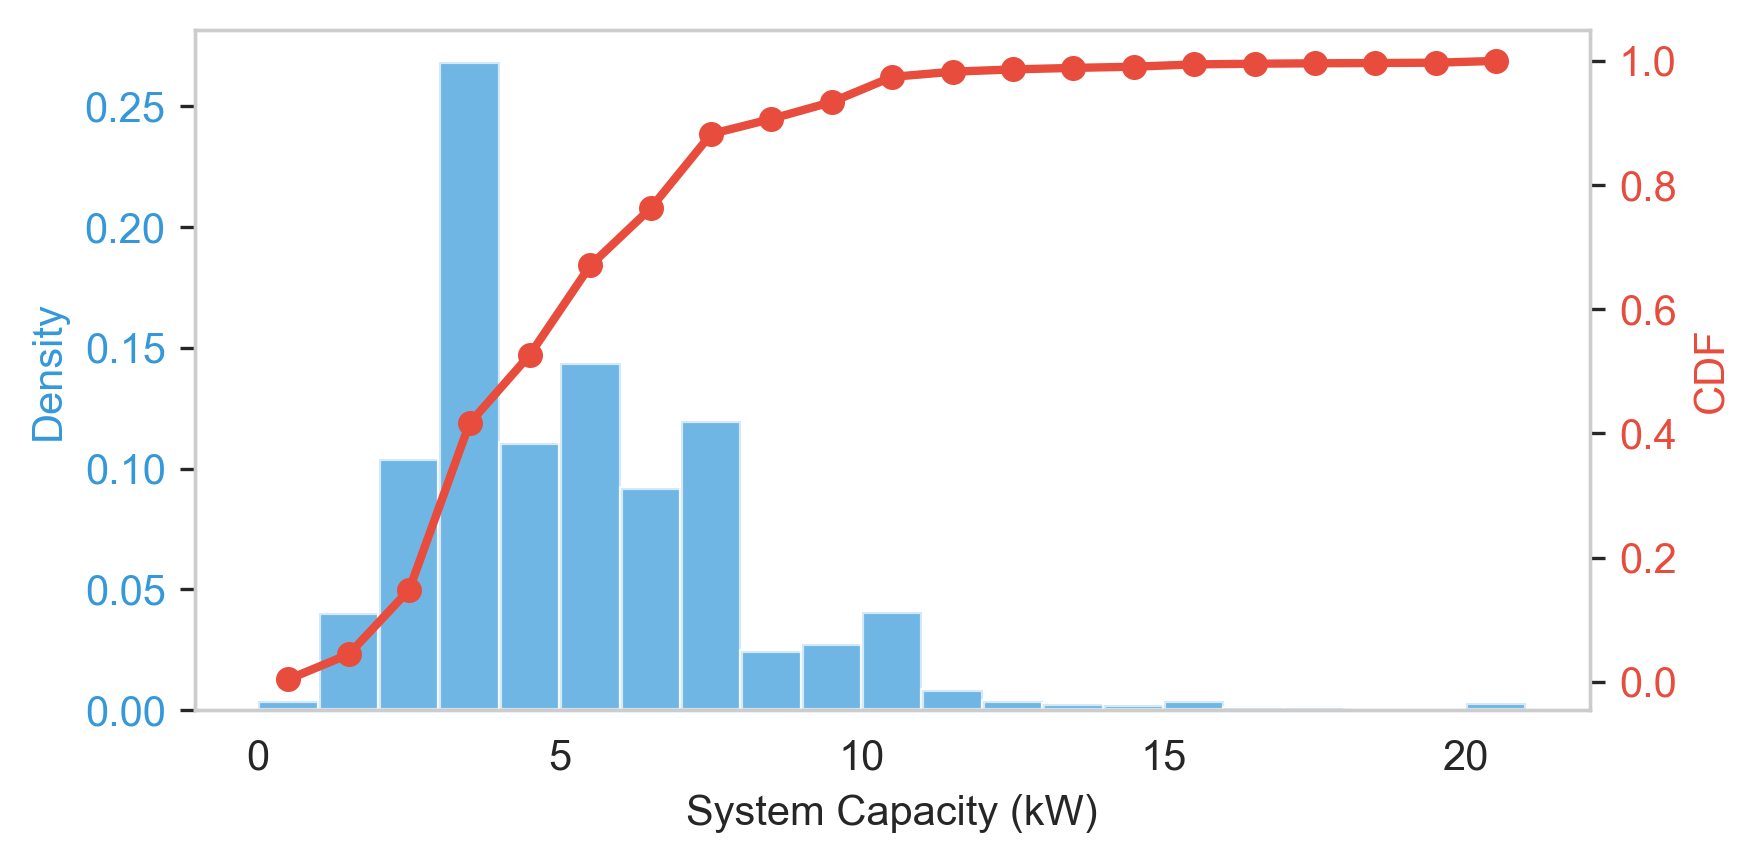
\includegraphics[width=1\textwidth]{figures/capacity_density_cdf.png}
    \caption{Distribution  of installed solar PV system capacity}
    \label{fig:capacity_density}
        \begin{flushleft}
        \footnotesize Note: Systems with capacity greater or equal to 20kW are grouped together. 
    \end{flushleft}
\end{figure}

The choice of system capacity can be influenced by many factors, including household size and utility incentives. \autoref{fig:capacity_size} depicts the relationship between installed system capacity (in kW) and the size of the living area of the home (in square feet), differentiated by utilities. It shows that as the housing size increases, the installed system capacity tends to increase. However, the intensity of this correlation varies by utility. Systems within the PNM service area have the highest slope compared to those served by EPE or other utilities. This difference could be attributed to variations in utility-level incentives (e.g., NEM policies) or correlations between utility service areas and other factors such as urban/rural or installer characteristics. It is notable that the shares of systems installed within the PNM, EPE, and other service areas are 77.9\%, 16.7\%, and 5.4\%, respectively.
 
\begin{figure}[!ht]
    \centering
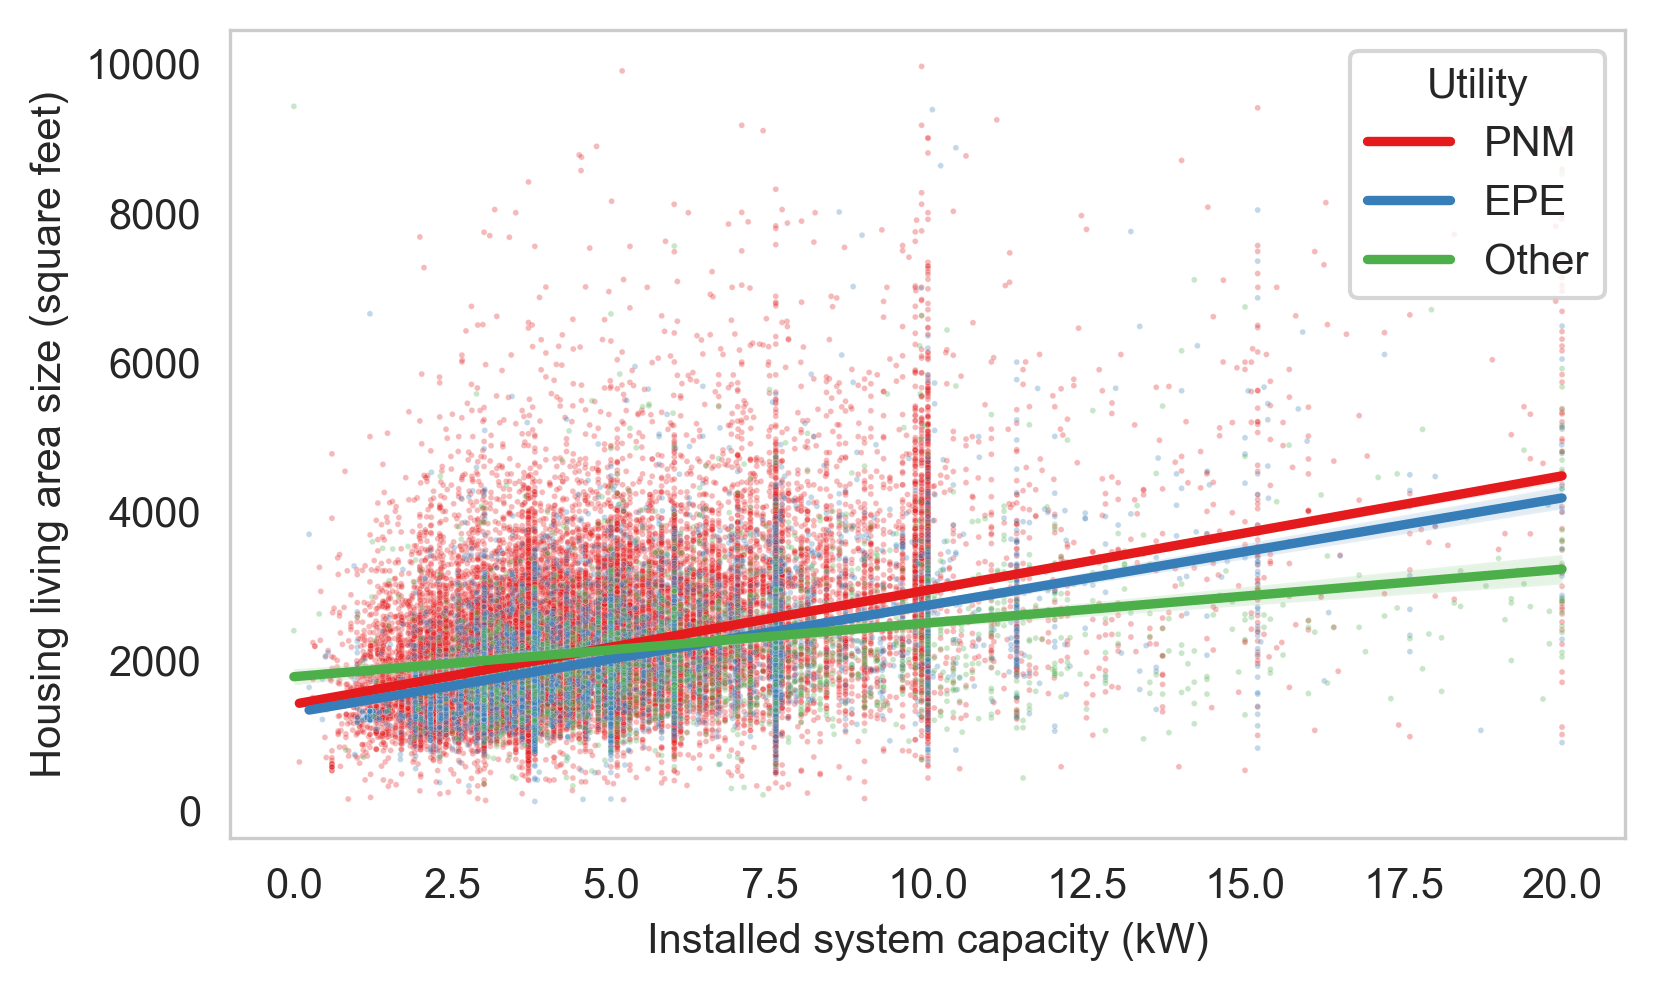
\includegraphics[width=1\textwidth]{figures/capacity_house_size.png}
    \caption{Linear relationship between installed capacity and housing size}
    \label{fig:capacity_size}
        \begin{flushleft}
        \footnotesize Note: Each colored dot in the graph represent on system within the corresponding utility service area. PNM stands for the Public Service Company of New Mexico, EPE stands for El Paso Electric, and Other includes all other utilities in NM.
    \end{flushleft}
\end{figure}

\autoref{fig:median_cap_map} shows the spatial distribution of median installed capacity. The map indicates that rural areas with low installation counts (\autoref{fig:installation_count}) tend to have higher median installed capacities.


\begin{figure}[!ht]
    \centering
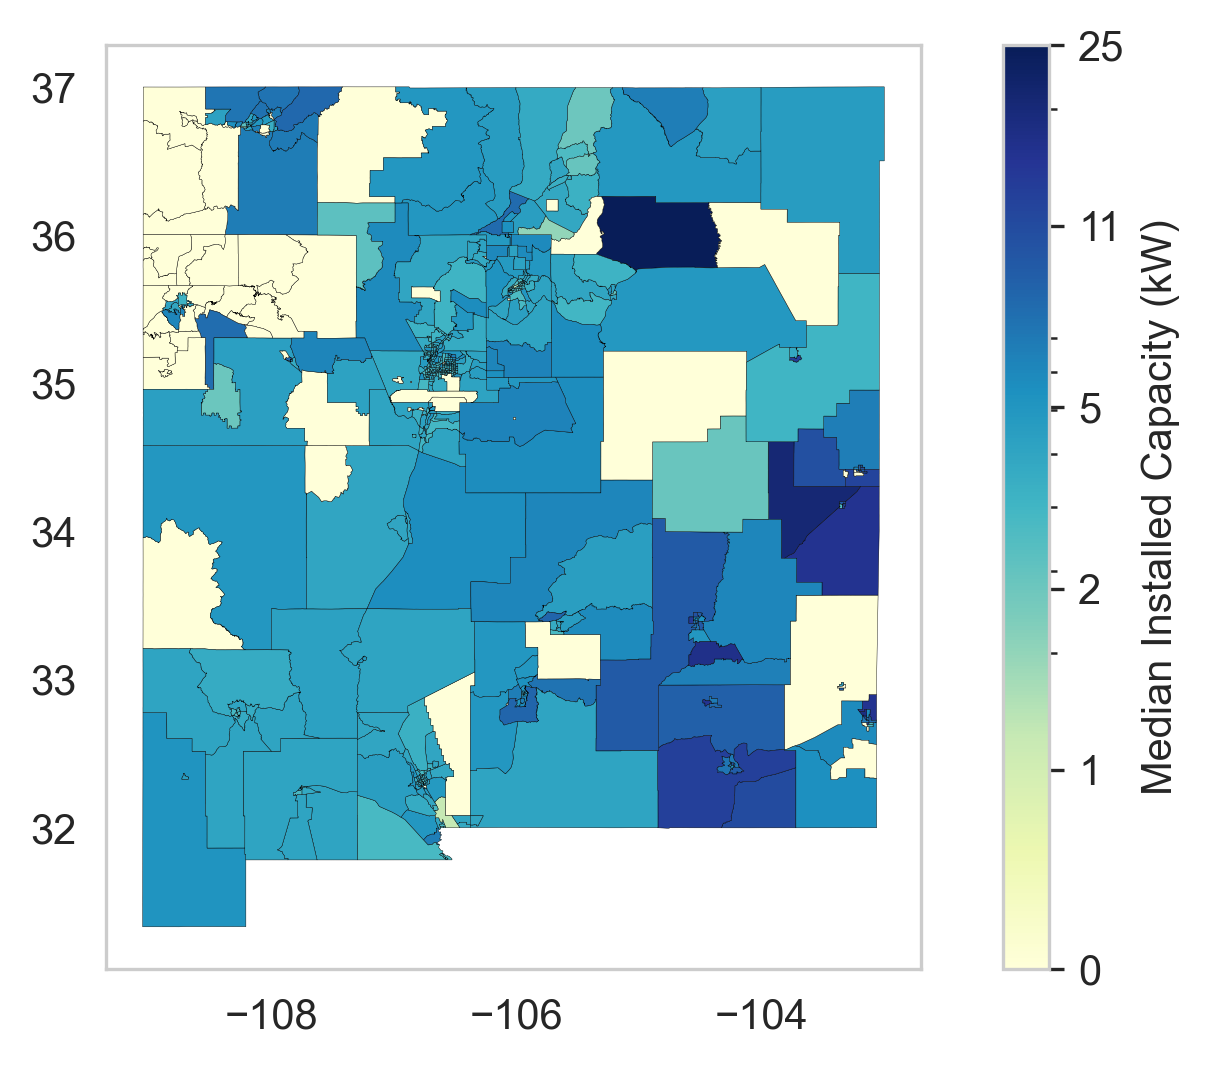
\includegraphics[width=0.7\textwidth]{figures/tract_median_capacity_map.png}
    \caption{Median system capacity by census tract}
    \label{fig:median_cap_map}
        \begin{flushleft}
        \footnotesize Note: The median system capacity for all installed systems within the census tract area. The census tracts areas are defined in the 2020 Decennial Census. The legend is in logarithm scale. 
    \end{flushleft}
\end{figure}


In summary, residential solar adoption in NM has grown exponentially since 2000, driven by decreasing solar panel costs and supportive tax incentives. However, this growth has been unevenly distributed across different geographical, income, and demographic groups. Urban areas, higher-income neighborhoods, and White-majority tracts have seen higher adoption rates compared to their rural, lower-income, and disadvantaged counterparts. The capacity of installed systems also varies, with larger systems more common in larger homes and areas with stronger utility incentives. These trends and distributions directly motivates the empirical analyses we carry out in the following sections.


%%%%%%%%%%%%%%%%%%%%%%%%%%%%%%%%%%%
\section{Adoption equity analysis}
% Section on the tract-level analysis

\subsection{Data}
The key variables we use in this part is the aggregate the count of newly installed residential solar PV systems each year at the census tract level. We merge the aggregated installation data with other census tract-level factors that may impact solar adoptions, including the percentage of White population, the percentage of Hispanic population, the percentage of population (25 years and over) with a bachelor’s degree or higher, median household income, and disadvantaged status. We also control for the other racial composition, housing characteristics, spatial weather, electricity providers and state credit incentives.

We conduct our analysis at the 2010 census tract level. New Mexico had 499 census tracts according to the 2010 Census, which increased to 612 by the 2020 Census. We normalize all data to the 2010 tract level to create a balanced panel dataset spanning from 2010 to 2022, which ensure the consistency and comparability of data across the entire study period.\footnote{Referring to the 2020 Census Redistricting Data (P.L. 94-171) Block Relationship files, details can be found here: \url{https://www.census.gov/geographies/reference-files/time-series/geo/relationship-files.2020.html}.} 

The dataset comprises 498 tracts in NM from 2010 through 2022. To avoid potential bias due to extreme outliers, we exclude one tract with a zero population across all study years. Table \ref{tab:datasource} provides detailed explanations of variables used in the empirical analysis and the respective data sources. Table \ref{tab:first-stage summary stat} presents summary statistics for the main variables over the sample period. 

The average residential solar PV installations per census tract-year is 6.33. The large standard deviations of income and housing value indicate significant variability across the dataset, suggesting a wide financial disparity where some individuals or groups have considerably higher incomes compared to others. For this reason, we take the logarithm of these variables in the regression analysis to account for their skewed distributions.


\begin{table}[htbp]
\caption{Summary of Measurements and Data Sources}
\label{tab:datasource}
\resizebox{\textwidth}{!}{%
\begin{tabular}{lll}
\hline
Variable & Measurements & Data sources \\ \hline
\multicolumn{3}{l}{\textit{\textbf{Dependent variables}}} \\
Count & Installed system count & EMNRD, NMPRC, and individual utilities \\ \hline
\multicolumn{3}{l}{\textit{\textbf{Explanatory variables}}} \\
Installation price & \begin{tabular}[c]{@{}l@{}}New Mexico average installation price, \\ cent/W\end{tabular} & Energy Information Administration \\
\textit{Housing characteristics} &  &  \\
Total housing unit & Total housing units & U.S. Census Bureau  (DP04)\\
Owner occupied & Owner occupied rate & U.S. Census Bureau (DP04) \\
Electricity & \begin{tabular}[c]{@{}l@{}}Share of of housing with electricity \\ as main heating source\end{tabular} & U.S. Census Bureau (B25040) \\
Built year group & \begin{tabular}[c]{@{}l@{}}Median housing age year group\\ Built after 2020 = 1;\\ Built between 2010 and 2019 = 2; \\ Built between 2000 and 2009 = 3; \\ Built between 1990 and 1999 = 4; \\ Built between 1980 and 1989 = 5, \\ Built between 1970 and 1979 = 6; \\ Built between 1960 and 1969 = 7; \\ Built between 1950 and 1959 = 8; \\ Built between 1940 and 1949 = 9; \\ Built in 1939 or earlier = 10.\end{tabular} & U.S. Census Bureau (DP04) \\
\textit{Racial composition} &  &  \\
Racial diversity & Racial diversity & Authors' compilation \\
White & Share of of White population & U.S. Census Bureau (DP05) \\
Hispanic & Share of of Hispanic population & U.S. Census Bureau (DP05) \\
\textit{Electricity provider variables} &  &  \\
Utility type & \begin{tabular}[c]{@{}l@{}}Electricity provider composition\\ IOU only = 1; \\ Cooperative only = 2; \\ Public utility only = 3; \\ IOU \& Cooperative = 4; \\ IOU \& Public utility = 5; \\ Cooperative \& Public utility = 6; \\ IOU \& Cooperative \& Public \\ utility = 7\end{tabular} & \begin{tabular}[c]{@{}l@{}}Homeland Infrastructure Foundation\\ -Level Data (HIFLD)\end{tabular} \\
PNM & \begin{tabular}[c]{@{}l@{}}Dummy for PNM service area\\ Yes = 1, other = 0\end{tabular} & \begin{tabular}[c]{@{}l@{}}Public Service Company of New \\ Mexico\end{tabular} \\
Electricity price & Average electricity price (cent/kWh) & \begin{tabular}[c]{@{}l@{}}U.S. Energy Information \\ Administration\end{tabular} \\
\textit{Weather variable} &  &  \\
Temperature & Average temperature & Solargis \\
GHI & Global Horizontal Irradiance (W/m$^2$) & Solargis \\
\textit{Other demographic variables} &  &  \\
Bachelor & \begin{tabular}[c]{@{}l@{}}Share of population (25 years and over)\\ with bachelor's or higher degree\end{tabular} & U.S. Census Bureau (S1501)\\
Income & \begin{tabular}[c]{@{}l@{}}Area median income \\ (inflation adjusted \$)\end{tabular} & U.S. Census Bureau (S1903) \\
Population & Total population & U.S. Census Bureau (DP05)\\
Disadvantage & Disadvantage rate & \begin{tabular}[c]{@{}l@{}}Climate and Economic Justice \\ Screening Tool\end{tabular} \\
Urban & Share of of urban housing units & U.S. Census Bureau (H2)\\
Credit & \begin{tabular}[c]{@{}l@{}}Dummy for state credit incentives\\ Yes = 1, other = 0\end{tabular} & Authors' compilation \\ \hline
\end{tabular}%
}
\end{table}






\begin{table}[!ht]
\centering
\caption{Summary statistics}
\label{tab:first-stage summary stat}
\resizebox{1\textwidth}{!}{%
\begin{tabular}{lrrrrrr}
\hline
\multicolumn{1}{r}{} & N & Mean & Std. Dev. & Median & Max & Min \\ \hline
Count & 6474 & 6.33 & 12.58 & 1 & 155 & 0 \\
%Occ & 6474 & 84.67 & 12.26 & 88.38 & 100 & 0 \\
Owner occupied & 6474 & 45.33 & 22.72 & 47.27 & 100 & 0 \\
%HHSize & 6474 & 2.68 & 0.75 & 2.59 & 21.38 & 0 \\
Electricity & 6474 & 17.64 & 14.86 & 12.21 & 100 & 0 \\
%MTG & 6474 & 28.06 & 14.51 & 26.36 & 81.12 & 0 \\
Built year group & 6474 & 5.18 & 1.45 & 5 & 10 & 1 \\
Utility type & 6474 & 2.72 & 1.71 & 2 & 6 & 1 \\
PNM & 6474 & 0.41 & 0.49 & 0 & 1 & 0 \\
Electricity price & 6474 & 13.01 & 1.83 & 13.08 & 21.11 & 7.78 \\
Installation price & 6474 & 5.68 & 1.33 & 5.30 & 9 & 4.30 \\
Temperature & 6474 & 14.03 & 2.83 & 14.40 & 18.90 & 3.68 \\
GHI & 6474 & 2034.01 & 59.10 & 2035.95 & 2189.54 & 1816.68 \\
%HSGrad & 6474 & 26.76 & 8.8 & 27.04 & 57.3 & 0 \\
Bachelor & 6474 & 25.92 & 16.48 & 21.95 & 81.78 & 0 \\
%HV & 6474 & 159112.05 & 114572.15 & 143100 & 851600 & 0 \\
Income & 6474 & 49333.93 & 21219.96 & 45054 & 174019.73 & 7278.34 \\
Population & 6474 & 4022.10 & 1805.60 & 3819 & 17497 & 71.02 \\
%Male & 6474 & 49.57 & 4.41 & 49.39 & 100 & 27.57 \\
Racial diversity & 6474 & 0.65 & 0.16 & 0.66 & 1 & 0.22 \\
White & 6474 & 72.31 & 21.71 & 78.43 & 100 & 0.16 \\
Non-Hispanic White & 6474 & 39.99 & 21.77 & 40.54 & 95.78 & 0 \\
Hispanic & 6474 & 45.82 & 23.42 & 44.31 & 100 & 0 \\
Total housing unit & 6474 & 1781.76 & 824.98 & 1680.50 & 8278 & 0 \\
Disadvantage & 6474 & 0.54 & 0.50 & 1 & 1 & 0 \\
Urban & 6474 & 73.28 & 38.64 & 98.08 & 100 & 0 \\
Credit & 6474 & 0.77 & 0.42 & 1 & 1 & 0 \\ \hline
\end{tabular}%
}
\end{table}




\begin{table}[!ht]
\caption{Summary statistics}
\label{tab: second-stage summary stat}
\resizebox{\textwidth}{!}{%
\begin{tabular}{lrrrrrr}
\hline
\multicolumn{1}{r}{} & N & Mean & Std. Dev. & Median & Max & Min \\ \hline
Count & 3849 & 10.64 & 14.84 & 5 & 155 & 1 \\
%Occ & 3849 & 87.58 & 10.23 & 90.41 & 100 & 28.83 \\
Owner occupied & 3849 & 48.94 & 22.95 & 51.7 & 95.45 & 0 \\
%HHSize & 3849 & 2.56 & 0.64 & 2.5 & 21.38 & 0 \\
Electricity & 3849 & 15.42 & 11.81 & 11.83 & 89.3 & 0 \\
%MTG & 3849 & 31.01 & 14.92 & 28.88 & 81.12 & 0 \\
Built year group & 3849 & 5.11 & 1.52 & 5 & 9 & 1 \\
Utility type & 3849 & 2.19 & 1.54 & 1 & 6 & 1 \\
PNM & 3849 & 0.55 & 0.5 & 1 & 1 & 0 \\
Electricity price & 3849 & 13.39 & 1.5 & 13.32 & 21.11 & 8.35 \\
Installation price & 3849 & 5.49 & 1.23 & 5.17 & 9 & 4.3 \\
Temperature & 3849 & 14.25 & 2.72 & 14.5 & 18.9 & 3.68 \\
GHI & 3849 & 2044.98 & 59.81 & 2046.8 & 2189.54 & 1816.68 \\
%HSGrad & 3849 & 24.26 & 8.58 & 24.2 & 55.48 & 1.17 \\
Bachelor & 3849 & 31.74 & 16.96 & 29.31 & 81.78 & 0.04 \\
%HV & 3849 & 191400.09 & 126224.39 & 169000 & 851600 & 0 \\
Income & 3849 & 54284.29 & 22928.66 & 49896 & 174019.73 & 7278.34 \\
Population & 3849 & 4257.71 & 1885.79 & 3977 & 17497 & 71.02 \\
%Male & 3849 & 49.1 & 3.75 & 49.11 & 87.52 & 27.57 \\
Racial diversity & 3849 & 0.65 & 0.15 & 0.66 & 1 & 0.25 \\
White & 3849 & 77.83 & 12.54 & 80.07 & 100 & 3.06 \\
Non-Hispanic White & 3849 & 43.27 & 20.02 & 44.01 & 90.48 & 0 \\
Hispanic & 3849 & 48.12 & 21.21 & 45.89 & 99.66 & 1.78 \\
Total housing unit & 3849 & 1897.37 & 800.37 & 1819.12 & 8278 & 24.06 \\
Disadvantage & 3849 & 0.42 & 0.49 & 0 & 1 & 0 \\
Urban & 3849 & 81.52 & 32.74 & 100 & 100 & 0 \\
Credit & 3849 & 0.77 & 0.42 & 1 & 1 & 0 \\ \hline
\end{tabular}%
}
\end{table}




\subsection{Empirical model}

We empirically investigate the disparity in solar PV adoptions across different demographic groups from two perspectives: 1) the impact of key factors on the extensive margin, which is the likelihood of solar PV adoption within census tracts over different years, and 2) the impact of key factors on the intensive margin, which represents the magnitude of solar PV installations.

To estimate adoption equity on the extensive margin, we use the aggregated installation data to generate a dependent variable as the indication of observing any solar adoption within a census tract-year. We compare the impact of various demographic and socioeconomic characteristics on the probability of having adoption through a linear probability regression with county and year fixed effects. Below is the model specification. Additionally, we use the fixed effect Logit model as a robustness check.



\begin{equation}
W_{it}= \beta_{0} + \beta_{1}H_{it} + \beta_{2}WH_{it} + \beta_{3}ln(INC_{it}) + \beta_{4}EDU_{it} + \beta_{5}DIS_{it} +\sum_{l}\gamma_{l}C_{it} + \lambda_{t} + \mu_{j} + \epsilon_{jt}
\end{equation}

\begin{math} W_{it} \end{math} is the binary variable indicating whether there is any solar adoption within census tract \begin{math} i \end{math} in year \begin{math} t \end{math}. We consider four key measurements from race, ethnicity, financial, and education perspectives. Specifically, \begin{math} H \end{math} represents the share of the Hispanic population, \begin{math} WH \end{math} represents the share of the White population, \begin{math} INC \end{math} is the area median household income, \begin{math} EDU \end{math} is the share of the population with a bachelor's degree or higher, and \begin{math} DIS \end{math} is a dummy variable indicating whether a census tract in year t is disadvantaged. \begin{math} C \end{math} is the vector of control variables, which includes average solar installation price, electricity providers, housing characteristics, weather, and state credit incentives. It also accounts for other unobserved policies and incentives at the county level through fixed effects.

Table \ref{tab: second-stage summary stat} presents summary statistics for the main variables, conditioned on having at least one installation within a tract-year over the sample period. The minimum installation count is 1, while the maximum is 155, with a standard deviation of 14.84. This substantial variability indicates that solar PV installations are not spatially uniform, reflecting disparities in adoption across different census tracts. We aim to estimate the effects of these key factors on the number of solar PV installations once adoption has occurred through a count model. 


\subsection{Results}


%%%%%%%%%%%%%%%%%%%%%%%%%%%%%%%%%%%
\newpage
\section{Distributional equity analysis}
% Section on credit claim

Another important aspect of solar equity is distributional equity, which pertains to whether the benefits of clean energy incentives are uniformly distributed across different demographic groups. In this section, we focus on the distributional equity of the state solar tax credit programs, SMDTC and NSMDTC, as they are the most prominent and salient forms of financial incentives for households. Given that solar tax credits are financed through tax dollars, understanding their distributional effects and potential regressivity is crucial for evaluating the effectiveness of these policies.

Our main research question is: Conditional on adopting solar, how do household and tract-level characteristics affect the probability of receiving state tax credits? Studying this question is crucial for several reasons. Firstly, it helps identify whether existing policies inadvertently favor certain demographic groups over others, which can exacerbate social inequalities. If solar incentives disproportionately benefit higher-income households or specific racial or ethnic groups, it indicates a need to redesign these policies to be more inclusive and equitable. Secondly, by understanding the factors that influence the distribution of these incentives, policymakers can develop targeted strategies to enhance the accessibility of solar energy for underrepresented and disadvantaged communities, contributing to a more just and sustainable energy transition. Lastly, evaluating the regressivity of solar tax credits ensures that public funds are used efficiently and equitably, promoting broader societal support for clean energy initiatives. Overall, this research provides valuable insights into designing more equitable and effective solar incentive programs.

\subsection{Data and descriptive analysis}

We use the system-level data described in section \ref{section:data_collect} for the years when tax credits were available (2006-2016 and after 2020). Since the demographics data spans from 2010 to 2022, we restrict our sample to the overlapping years: 2010-2016 and 2020-2022. \autoref{fig:credit_claim} shows the number of newly installed systems each year that received or did not receive solar tax credits within PNM, EPE, SEC, and LADPU service areas. It also shows the total credit amount claimed each year by all residential solar systems. During the first phase of the tax credit program (SMDTC), the majority of installations benefited from the 10\% credit. In contrast, in the second phase (NSMDTC), more than half of the installations did not receive the credit. This gap can partially be explained by the annual funding cap implemented with NSMDTC. In 2020 and 2021, the cap was \$8 million, increasing to \$12 million in 2022 and 2023.\footnote{In 2024, Governor Lujan Grisham signed House Bill 252 into law to raise the annual aggregate cap to \$30 million per year \parencite{newsolarcap}.} The aggregate cap was reached in 2021 and 2022, resulting in 190 and 226 tax credit application rejections, respectively.

\begin{figure}[H]
    \centering
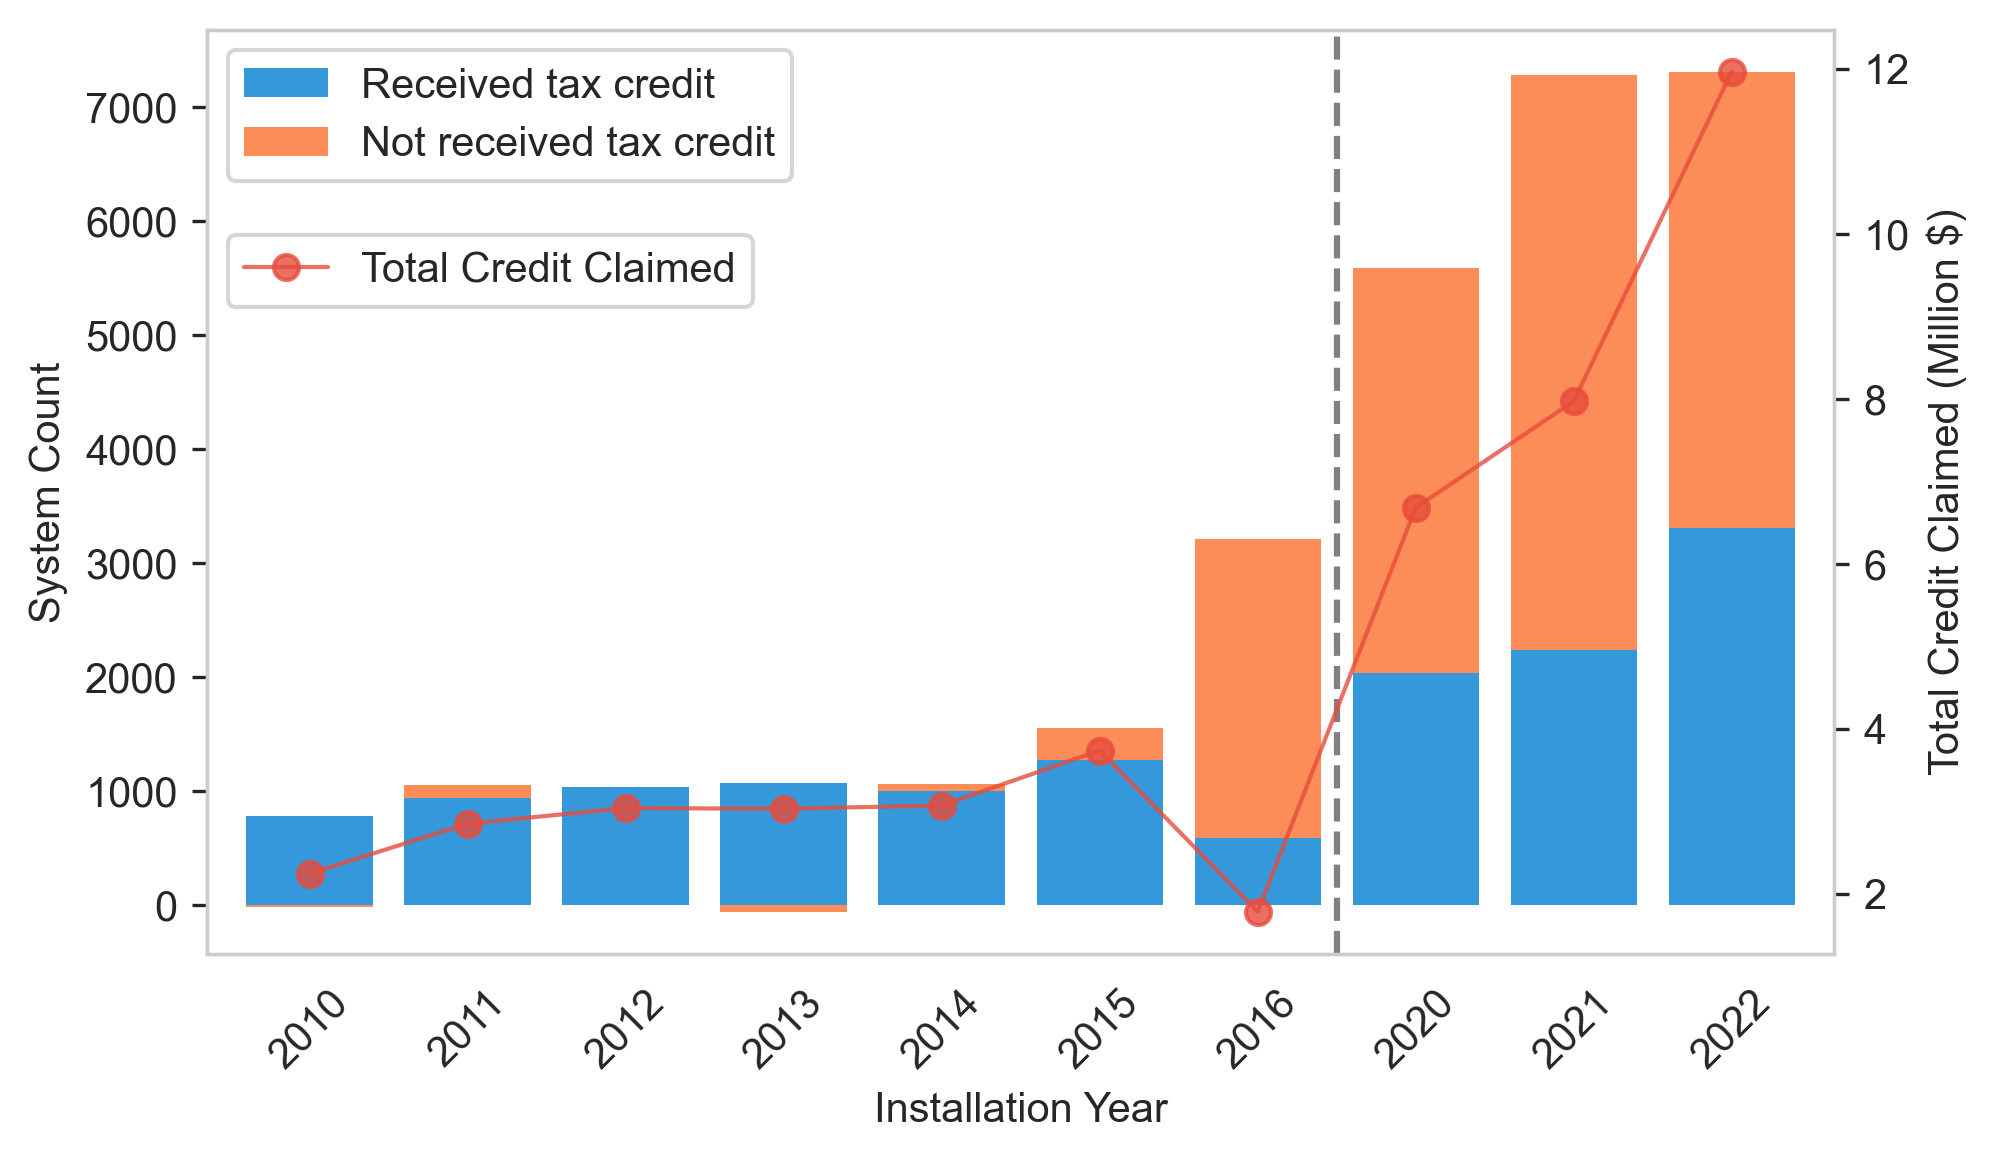
\includegraphics[width=0.9\textwidth]{figures/credit_claim.png}
    \caption{Installed systems by credit claim status and total credit claimed between 2010 and 2022}
    \label{fig:credit_claim}
      \begin{flushleft}
        \footnotesize Note: The total system counts only include systems within PNM, EPE, SEC, and LADPU service areas. The number of systems receiving credits is also for this subset of utilities only. The total credit claimed accounts for all residential systems. In 2010 and 2013, the number of systems that did not receive tax credits (orange bars) was negative. This could be due to data errors between different data sources or credit claim delays.
    \end{flushleft}
\end{figure}

\autoref{fig:credit_map} illustrates the concentration of total tax credit claims and the average amount claimed per system. Total credits concentrate in census tracts with high solar installations (\autoref{fig:tract_map}). In contrast, the average tax credit is highly correlated with the median installed capacity of the tract (\autoref{fig:median_cap_map}).

\begin{figure}[H]
    \centering
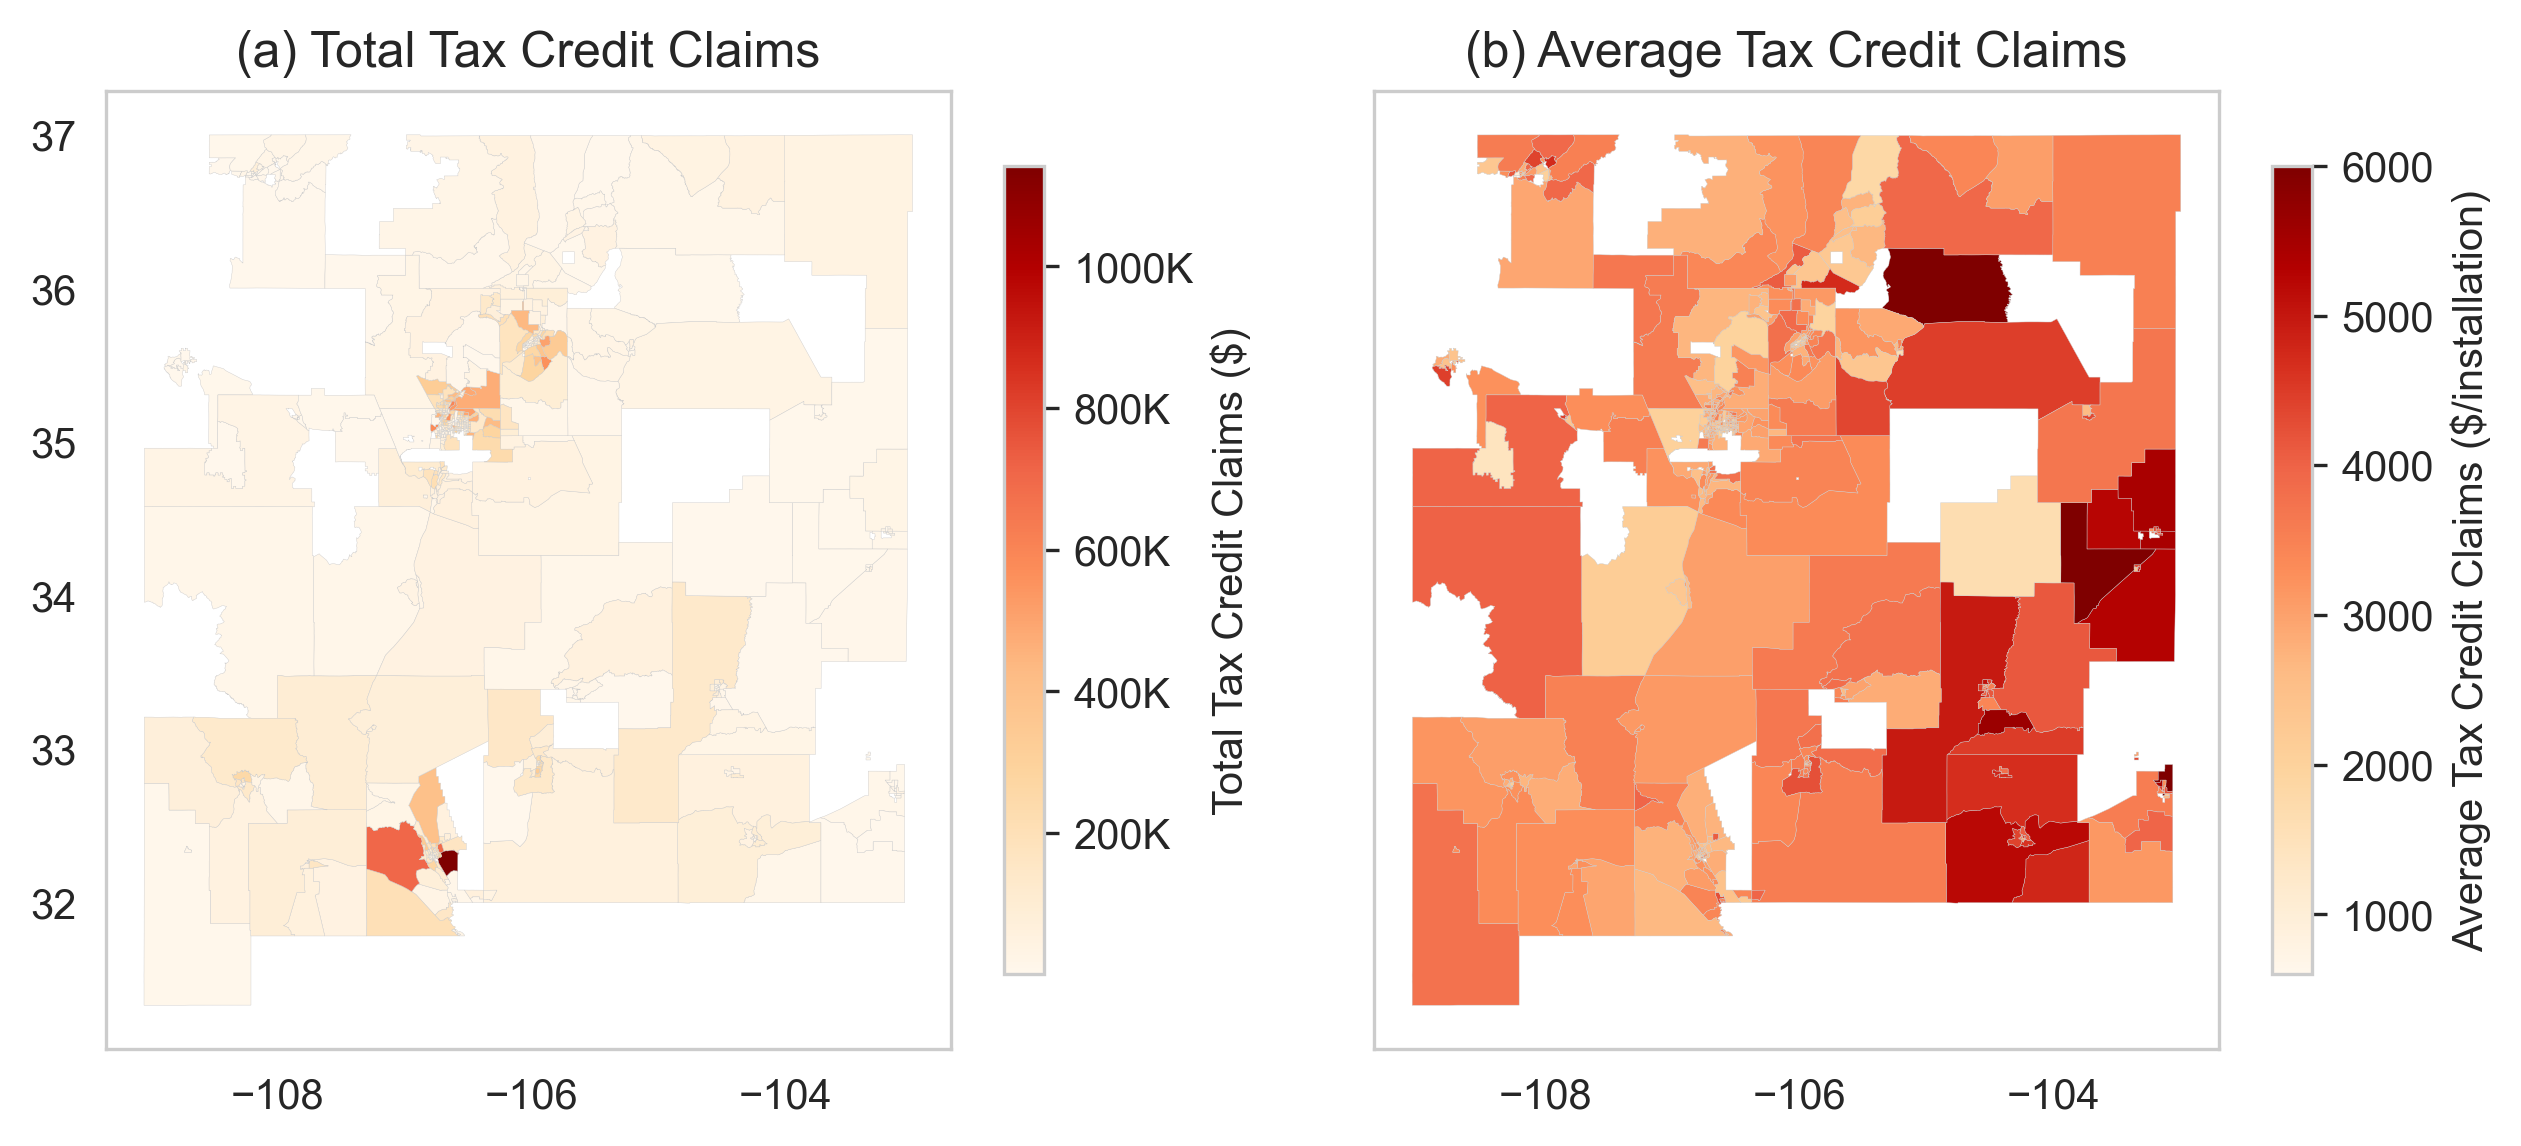
\includegraphics[width=1\textwidth]{figures/credit_claim_maps.png}
    \caption{Total and average tax credit claim by census tract}
    \label{fig:credit_map}
      \begin{flushleft}
        \footnotesize Note: The total credit claimed sums up all historical amounts of credit received in the census tract by 2022. The average credit claim uses the total amount divided by the number of systems that received tax credits.
    \end{flushleft}
\end{figure}

To answer the research question, we need to match the two data sources of solar installations to identify which systems received solar credits. The EMNRD data contains a wealth of information but only for systems that received tax credits, while the utility data includes the universe of all systems installed. We match the recorded address of the installed systems. Since the recorded address for the same system may vary across datasets, some of the systems in the EMNRD data cannot be found in the utility dataset despite our best efforts. \autoref{tab:compare_emnrd_utility} shows the result of the matching, which, although imperfect, remains statistically insignificant.


\autoref{tab:sumstat} shows the summary statistics of the matched dataset, and \autoref{fig:corr_matrix} displays the correlation matrix of the key variables.


\begin{table}[!ht]
    \centering
    \caption{Summary statistics}
    \resizebox{1\textwidth}{!}{
   \begin{tabular}{lrrrrr}
\hline
                                         &   N &      Mean &       Std. Dev. &   Min &      Max \\
\hline
 State credit                            &   26735 &      0.44 &      0.50 &     0 &        1 \\
 System capacity                         &   26735 &      5.09 &      2.51 &     0 &       43 \\
 \# of Bedrooms                           &   25951 &      3.33 &      0.78 &     0 &       17 \\
 Zestimate                               &   26087 & 483442.77 & 348557.87 & 49600 & 14324300 \\
 Housing size (sq ft)                    &   26735 &   2201.28 &    975.74 &   100 &    24517 \\
 Year built                              &   26397 &   1989.18 &     21.99 &  1750 &     2024 \\
 \% population with bachelor degree (\ensuremath{>}25) &   26735 &      0.37 &      0.17 &     0 &        0 \\
 Owner occupancy rate                    &   26735 &      0.61 &      0.23 &     0 &        1 \\
 Mortgage rate                           &   26735 &      0.41 &      0.17 &     0 &        0 \\
 Area Median Income                      &   26735 &  69062.99 &  27312.01 & 12014 &   250000 \\
 Population                              &   26735 &   4904.32 &   2235.43 &   274 &    15722 \\
 Median Age                              &   26735 &     41.07 &      8.80 &    20 &       82 \\
 \% population identified as White        &   26735 &      0.83 &      0.09 &     0 &        1 \\
 \% population identified as Hispanic     &   26735 &      0.47 &      0.21 &     0 &        1 \\
 Urban share                             &   26735 &      0.86 &      0.28 &     0 &        1 \\
 Within disadvantaged census tracts      &   26735 &      0.26 &      0.44 &     0 &        1 \\
\hline
\end{tabular}}
    
    \label{tab:sumstat}
\end{table}

\subsection{Determinants for tax credit claim}

The dependent variable is whether a household received  tax credit upon solar adoption. The linear probability model is sufficient to estimate the effect of various household and tract-level characteristics on the probably of credit claim.


\begin{table}[!ht] \centering
  \caption{Regression results of linear probability model for state credit claim}
  \resizebox{1\textwidth}{!}{
\begin{tabular}{@{\extracolsep{5pt}}lccccc}
\\[-1.8ex]\hline
\hline \\[-1.8ex]
& \multicolumn{5}{c}{\textit{Dependent variable: State Credit}} \
\cr \cline{2-6}
\\[-1.8ex] & (1) & (2) & (3) & (4) & (5) \\
\hline \\[-1.8ex]
 System capacity & -0.006$^{***}$ & 0.003$^{*}$ & 0.010$^{***}$ & 0.009$^{***}$ & 0.008$^{***}$ \\
& (0.001) & (0.001) & (0.001) & (0.001) & (0.001) \\
 Log Zestimate & 0.301$^{***}$ & 0.148$^{***}$ & 0.117$^{***}$ & 0.134$^{***}$ & 0.156$^{***}$ \\
& (0.009) & (0.012) & (0.011) & (0.012) & (0.015) \\
 Year built & -0.002$^{***}$ & -0.000$^{}$ & -0.001$^{***}$ & -0.001$^{***}$ & -0.001$^{***}$ \\
& (0.000) & (0.000) & (0.000) & (0.000) & (0.000) \\
 Log Housing size (sq ft) & 0.004$^{}$ & 0.029$^{*}$ & 0.004$^{}$ & -0.005$^{}$ & -0.016$^{}$ \\
& (0.012) & (0.014) & (0.013) & (0.013) & (0.015) \\
 \# of Bedrooms & & -0.017$^{***}$ & -0.009$^{*}$ & -0.010$^{*}$ & -0.010$^{*}$ \\
& & (0.005) & (0.004) & (0.004) & (0.004) \\
 \% population with bachelor degree ($>$25) & & 0.183$^{***}$ & 0.260$^{***}$ & 0.213$^{***}$ & 0.187$^{***}$ \\
& & (0.033) & (0.031) & (0.034) & (0.037) \\
 Owner occupancy rate & & -0.383$^{***}$ & 0.141$^{***}$ & 0.136$^{***}$ & 0.139$^{***}$ \\
& & (0.021) & (0.025) & (0.025) & (0.025) \\
 Mortgage rate & & -0.298$^{***}$ & -0.287$^{***}$ & -0.272$^{***}$ & -0.228$^{***}$ \\
& & (0.031) & (0.030) & (0.031) & (0.031) \\
 Log Area Median Income & & 0.067$^{***}$ & -0.015$^{}$ & -0.005$^{}$ & -0.005$^{}$ \\
& & (0.014) & (0.014) & (0.014) & (0.014) \\
 Log Population & & 0.054$^{***}$ & 0.016$^{*}$ & 0.015$^{*}$ & 0.024$^{**}$ \\
& & (0.007) & (0.007) & (0.007) & (0.007) \\
 Log Median Age & & 0.048$^{*}$ & 0.009$^{}$ & 0.008$^{}$ & 0.023$^{}$ \\
& & (0.022) & (0.021) & (0.021) & (0.021) \\
 \% population identified as White & & 0.064$^{}$ & 0.017$^{}$ & -0.011$^{}$ & -0.067$^{}$ \\
& & (0.038) & (0.036) & (0.038) & (0.040) \\
 \% population identified as Hispanic & & -0.090$^{***}$ & -0.105$^{***}$ & -0.145$^{***}$ & -0.142$^{***}$ \\
& & (0.024) & (0.023) & (0.025) & (0.029) \\
 Urban share & & -0.061$^{***}$ & -0.031$^{**}$ & -0.021$^{}$ & -0.008$^{}$ \\
& & (0.012) & (0.011) & (0.012) & (0.012) \\
 With in disadvantaged census tracts & & -0.039$^{***}$ & -0.034$^{***}$ & -0.032$^{***}$ & -0.042$^{***}$ \\
& & (0.009) & (0.009) & (0.009) & (0.009) \\
 Year Fixed Effects & No & No & Yes & Yes & Yes \\
 Utility Fixed Effects & No & No & No & Yes & No \\
 County Fixed Effects & No & No & No & No & Yes \\
\hline \\[-1.8ex]
 Observations & 25779 & 25234 & 25234 & 25234 & 25234 \\
 $R^2$ & 0.085 & 0.157 & 0.232 & 0.233 & 0.235 \\
 Adjusted $R^2$ & 0.084 & 0.156 & 0.231 & 0.232 & 0.234 \\
 Residual Std. Error & 0.475 & 0.456 & 0.435 & 0.435 & 0.435 \\
 F Statistic & 594.858$^{***}$ & 313.067$^{***}$ & 317.205$^{***}$ & 282.905$^{***}$ & 209.254$^{***}$ \\
\hline
\hline \\[-1.8ex]
\textit{Note:} & \multicolumn{5}{r}{$^{*}$p$<$0.05; $^{**}$p$<$0.01; $^{***}$p$<$0.001} \\
\end{tabular}
}
\end{table}







Result by SMDTC round

\begin{table}[!ht] \centering
  \caption{Regression results of linear probability model for state credit claim for each round of SMDTC}
  \resizebox{0.7\textwidth}{!}{
\begin{tabular}{@{\extracolsep{5pt}}lcc}
\\[-1.8ex]\hline
\hline \\[-1.8ex]
& \multicolumn{2}{c}{\textit{Dependent variable: State Credit}} \
\cr \cline{2-3}
\\[-1.8ex] & \multicolumn{1}{c}{First round} & \multicolumn{1}{c}{Second round}  \\
  & (before 2016) & (after 2020) \\
\hline \\[-1.8ex]
 System capacity & 0.002$^{}$ & 0.010$^{***}$ \\
& (0.002) & (0.002) \\
 Log Zestimate & 0.024$^{}$ & 0.251$^{***}$ \\
& (0.021) & (0.020) \\
 Year built & -0.001$^{**}$ & -0.001$^{***}$ \\
& (0.000) & (0.000) \\
 Log Housing size (sq ft) & 0.033$^{}$ & -0.062$^{**}$ \\
& (0.021) & (0.020) \\
 \# of Bedrooms & 0.004$^{}$ & -0.016$^{**}$ \\
& (0.007) & (0.006) \\
 \% population with bachelor degree ($>$25) & 0.207$^{**}$ & 0.170$^{***}$ \\
& (0.065) & (0.045) \\
 Owner occupancy rate & 0.091$^{**}$ & 0.026$^{}$ \\
& (0.033) & (0.048) \\
 Mortgage rate & -0.300$^{***}$ & -0.095$^{}$ \\
& (0.047) & (0.051) \\
 Log Area Median Income & 0.026$^{}$ & -0.008$^{}$ \\
& (0.023) & (0.019) \\
 Log Population & 0.028$^{*}$ & 0.024$^{*}$ \\
& (0.012) & (0.010) \\
 Log Median Age & 0.182$^{***}$ & -0.003$^{}$ \\
& (0.035) & (0.029) \\
 \% population identified as White & -0.252$^{***}$ & 0.007$^{}$ \\
& (0.069) & (0.051) \\
 \% population identified as Hispanic & -0.004$^{}$ & -0.152$^{***}$ \\
& (0.052) & (0.036) \\
 Urban share & 0.007$^{}$ & -0.033$^{*}$ \\
& (0.019) & (0.016) \\
 With in disadvantaged census tracts & -0.006$^{}$ & -0.038$^{***}$ \\
& (0.016) & (0.011) \\
 Year Fixed Effects & Yes & Yes \\
 County Fixed Effects & Yes & Yes \\
\hline \\[-1.8ex]
 Observations & 8326 & 16908 \\
 $R^2$ & 0.382 & 0.112 \\
 Adjusted $R^2$ & 0.380 & 0.111 \\
 Residual Std. Error & 0.386 & 0.453 \\
 F Statistic & 160.188$^{***}$ & 71.071$^{***}$ \\
\hline
\hline \\[-1.8ex]
\textit{Note:} & \multicolumn{2}{r}{$^{*}$p$<$0.05; $^{**}$p$<$0.01; $^{***}$p$<$0.001} \\
\end{tabular}}
\end{table}


\newpage
%%%%%%%%%%%%%%%%%%%%%%%%%%%%%%%%%%%
\section[Conclusion]{Conclusion and policy implications}



%%%%%%%%%%%%%%%%%%%%%%%%%%%%%%%%%%%
\newpage
\appendix
\numberwithin{equation}{section}
\numberwithin{figure}{section}
\numberwithin{table}{section}
\section[Appendix]{Appendix}

\begin{figure}[H]
    \centering
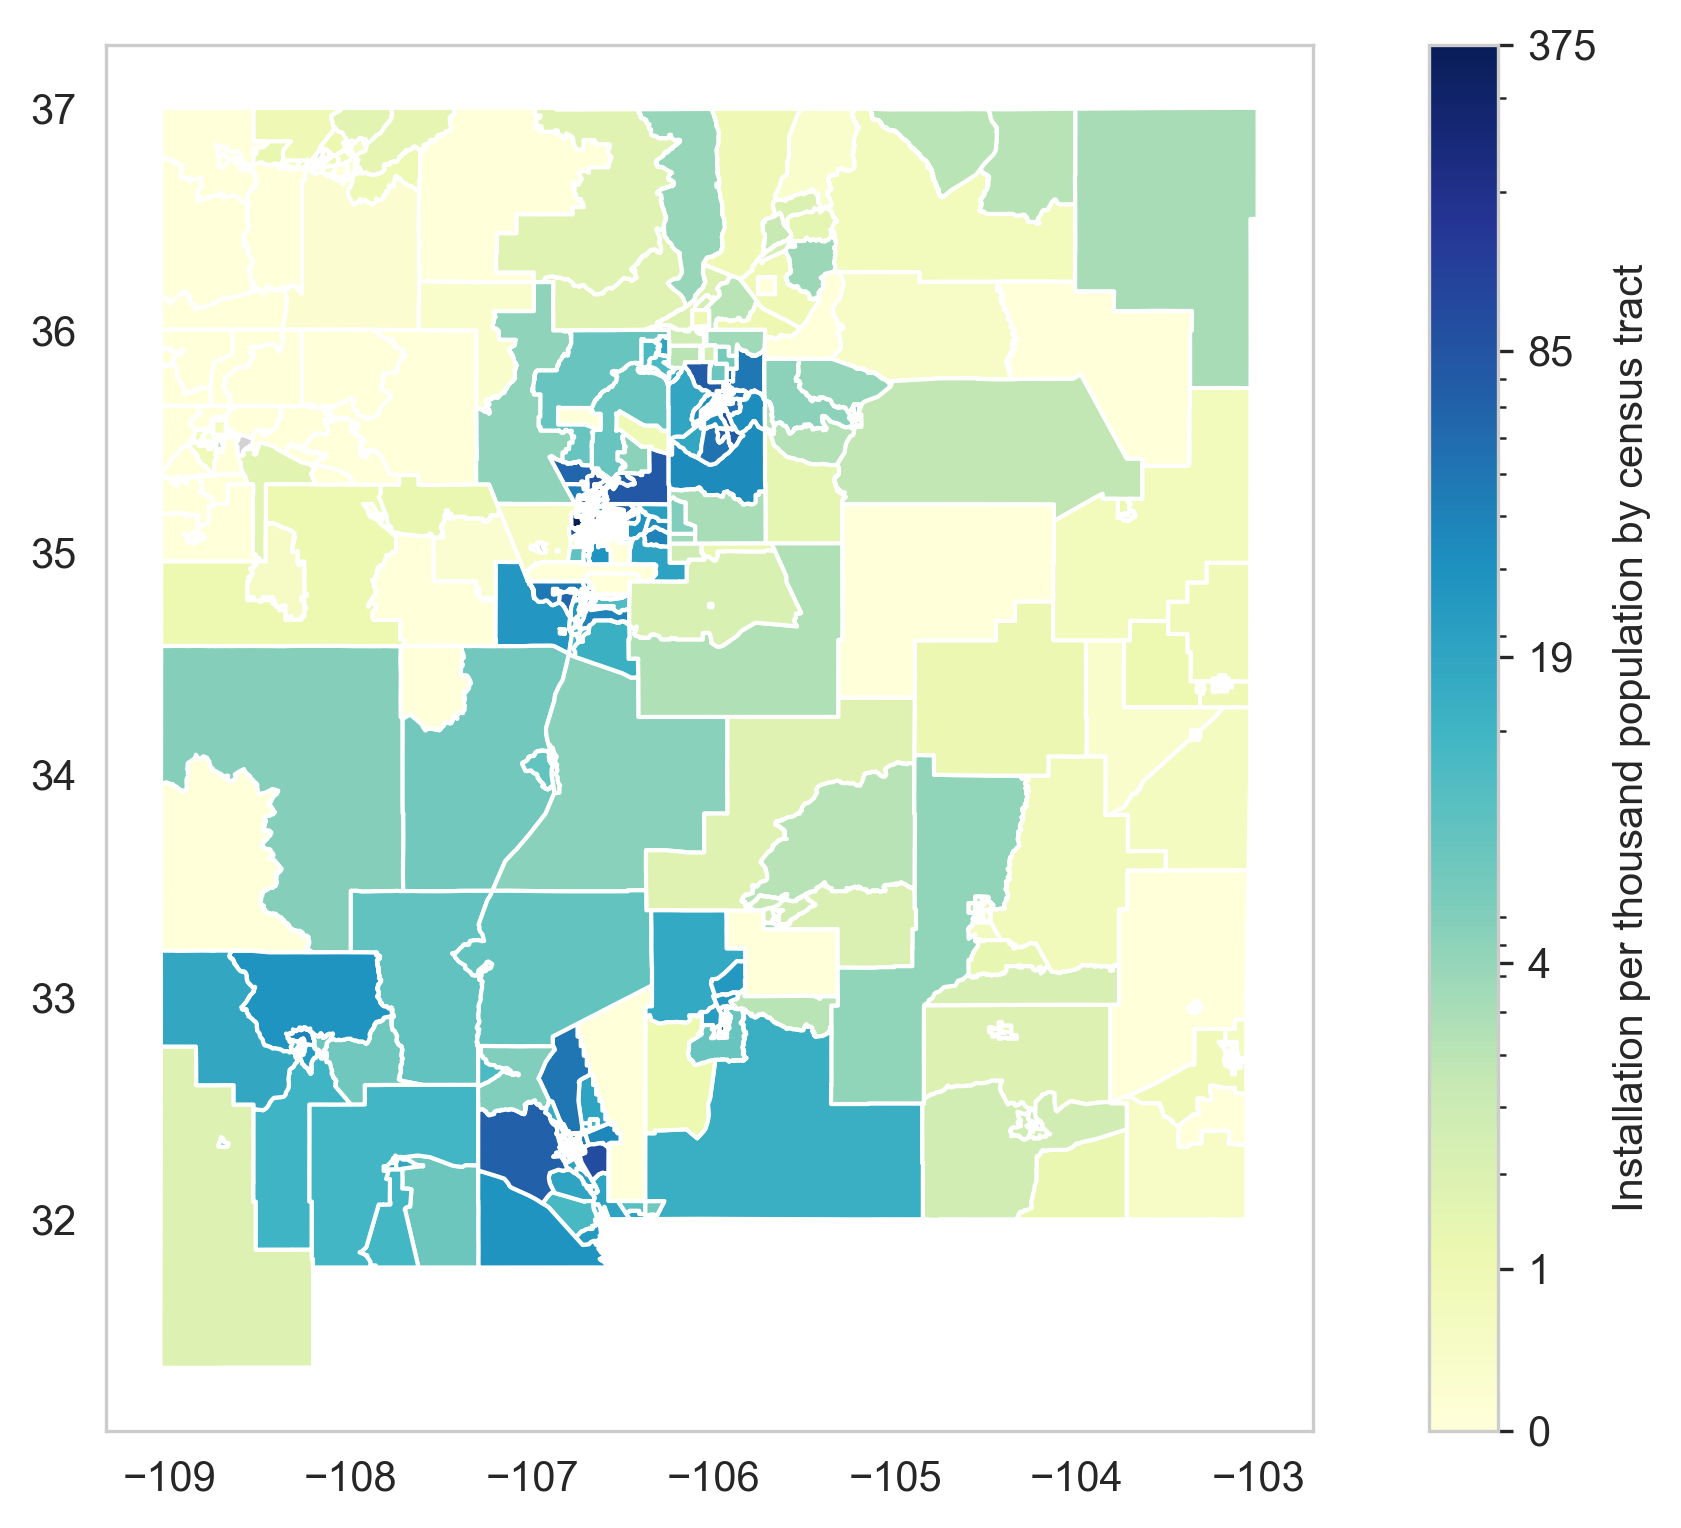
\includegraphics[width=0.8\textwidth]{figures/tract_count_per_kpop_map.png}
    \caption{Installation per thousand people by 2020 census tract}
    \label{fig:install_kpop}
      \begin{flushleft}
        \footnotesize Note: The total installation count is up to the end of 2023 for each census tract. The census tracts areas are defined in the 2020 Decennial Census. The tract-level population is taken at the 2022 level from the American Community Survey 1-year data. The legend is in logarithm scale. 
    \end{flushleft}
\end{figure}

\begin{figure}[!ht]
    \centering
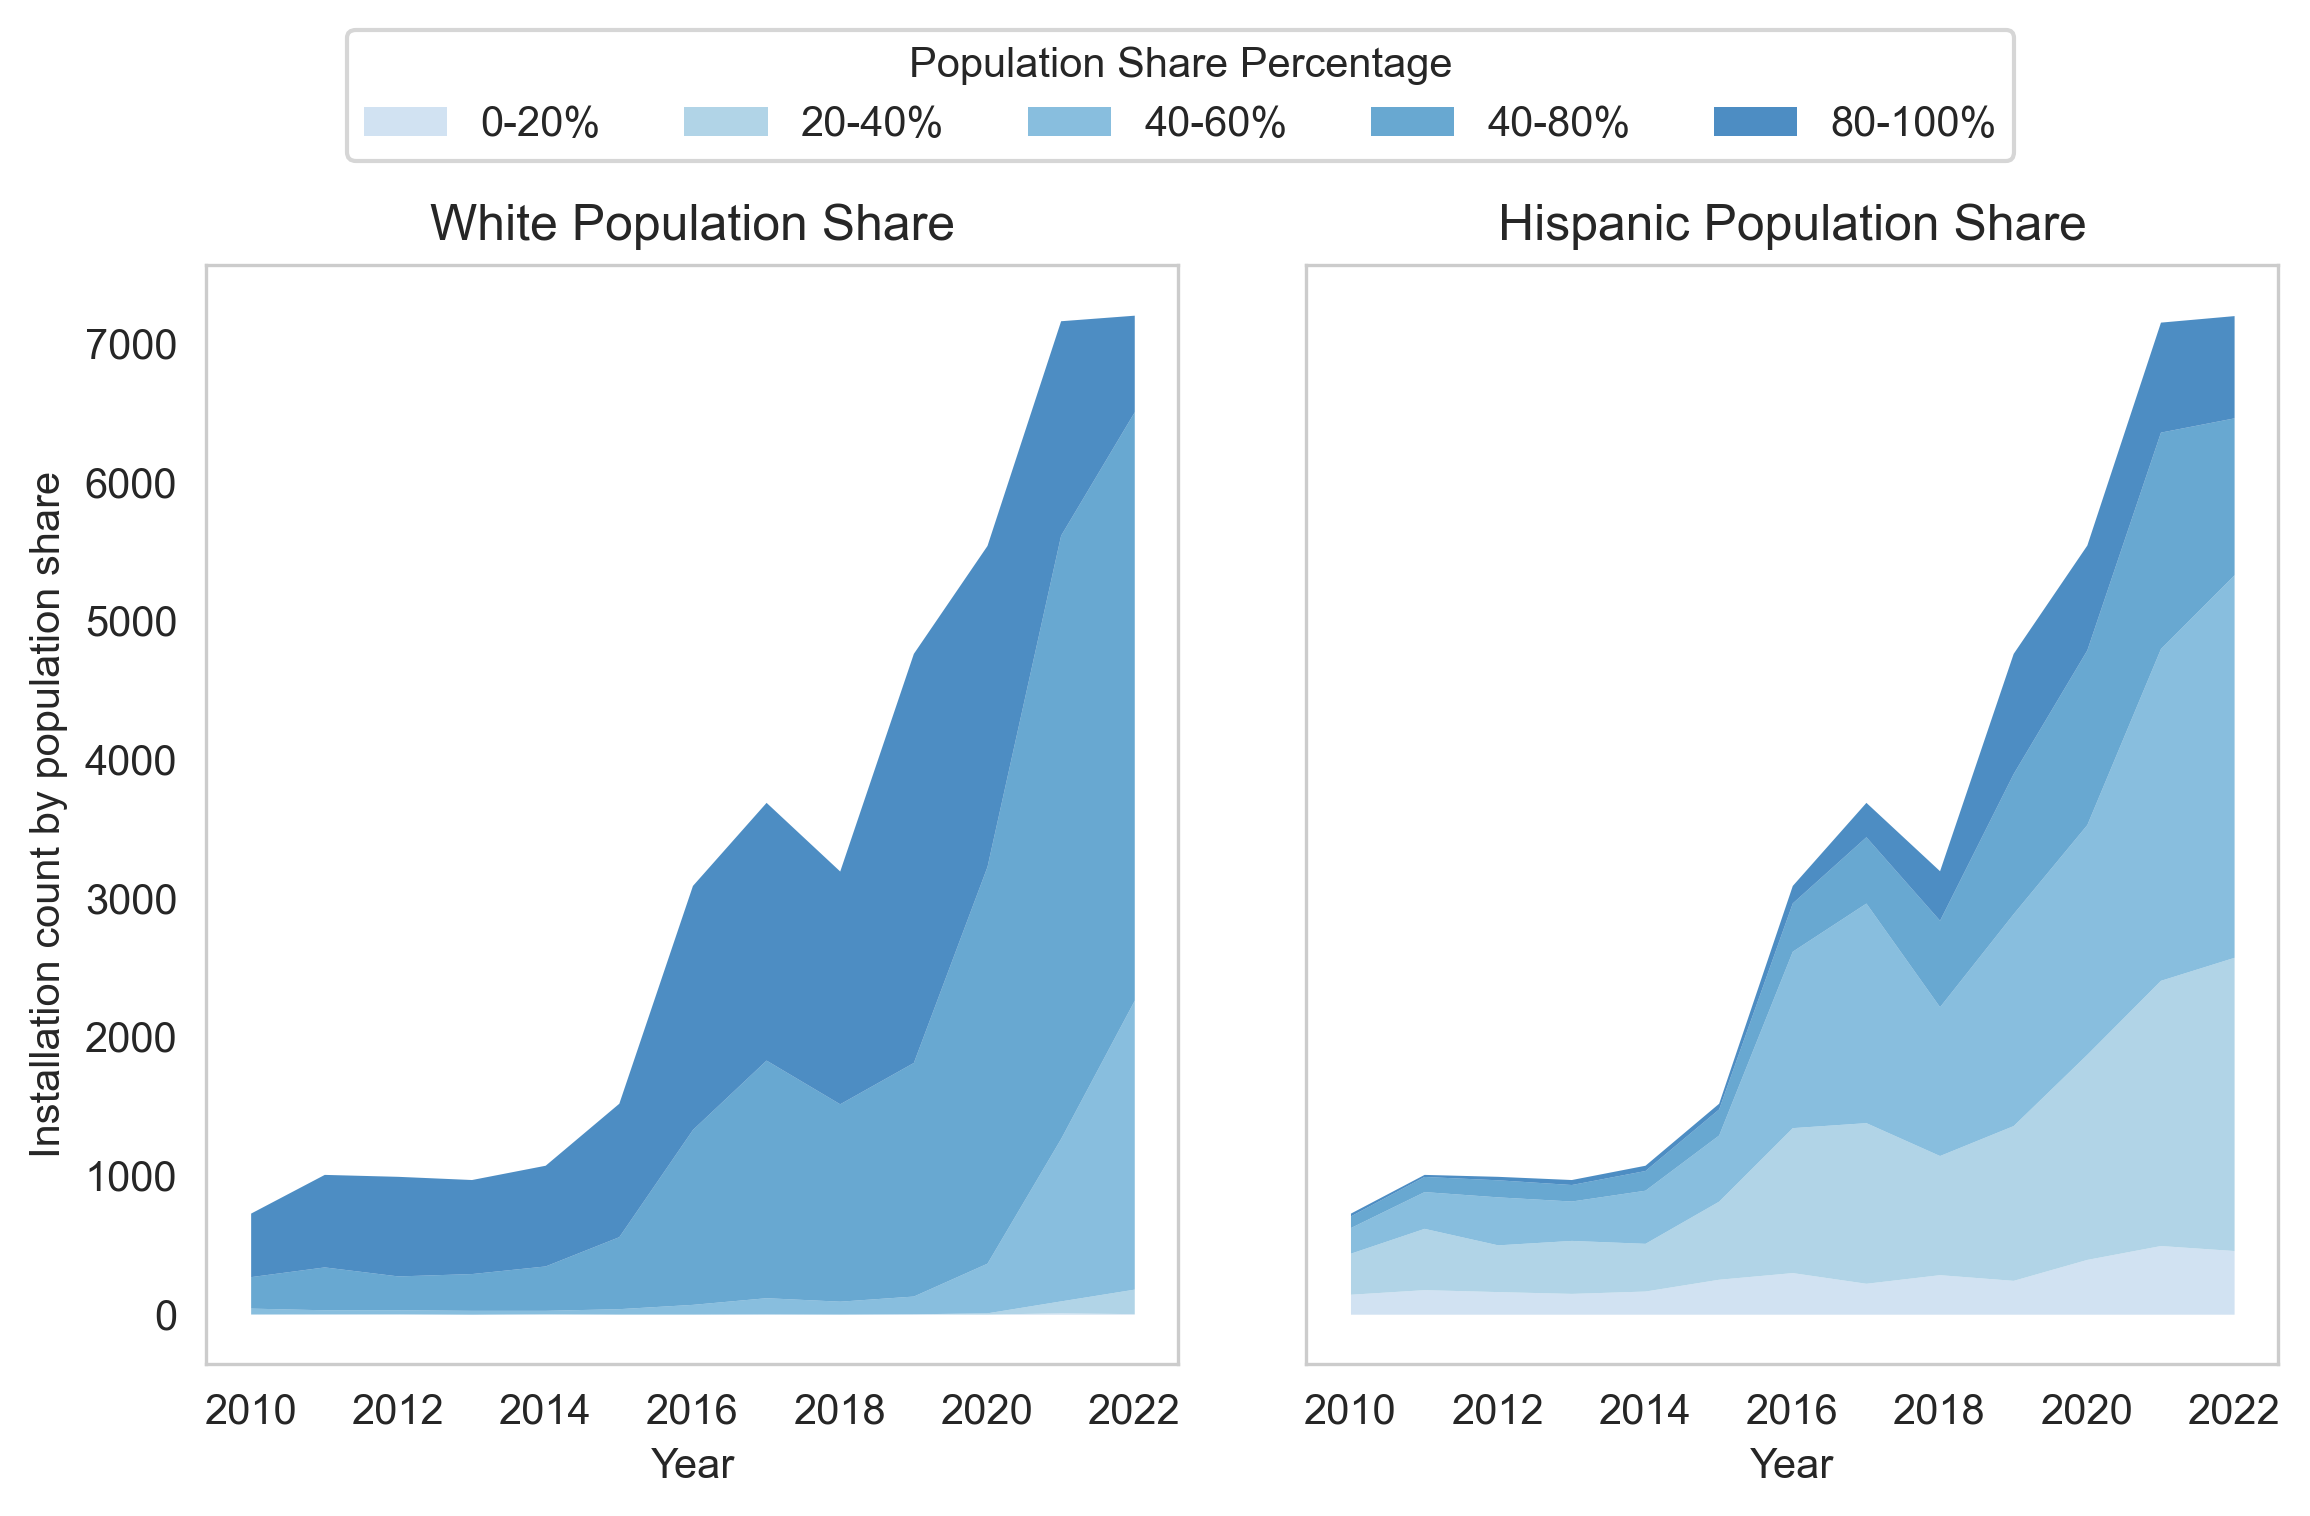
\includegraphics[width=1\textwidth]{figures/population_quintiles.png}
    \caption{Installation by racial population share}
    \label{fig:population_quintiles}
    %     \begin{flushleft}
    %     \footnotesize Note: White majority refers to census tracts with more than 50\% population identified as white. Hispanic majority refers to census tracts with more than 50\% population identified as Hispanic. 
    % \end{flushleft}
\end{figure}


\begin{table}[H] 
\caption{Comparison of systems claimed tax credit in the EMNRD and utility datasets}
\label{tab:compare_emnrd_utility}
\centering
\begin{tabular}{lrrr}
\toprule
Utility & EMNRD Count & Utility Claim Count & Difference \\
\midrule
PNM & 14350 & 13435 & -915 \\
EPE & 3322 & 2866 & -456 \\
SEC & 91 & 72 & -19 \\
LADPU & 207 & 193 & -14 \\
\bottomrule
\multicolumn{4}{l}{\textit{Note:  T-statistic: 0.0759, P-value: 0.9419}} \\
\end{tabular}


\begin{flushleft}\footnotesize{Notes: The t-test compares the mean counts of tax credit claims between the EMNRD dataset and the utility datasets (PNM, EPE, SEC, LADPU) where state credit is claimed. The result suggests that the number of tax credit claims recorded in the EMNRD dataset is not significantly different from those recorded in the utility datasets.}
\end{flushleft}
\end{table}

\begin{figure}[H]
    \centering
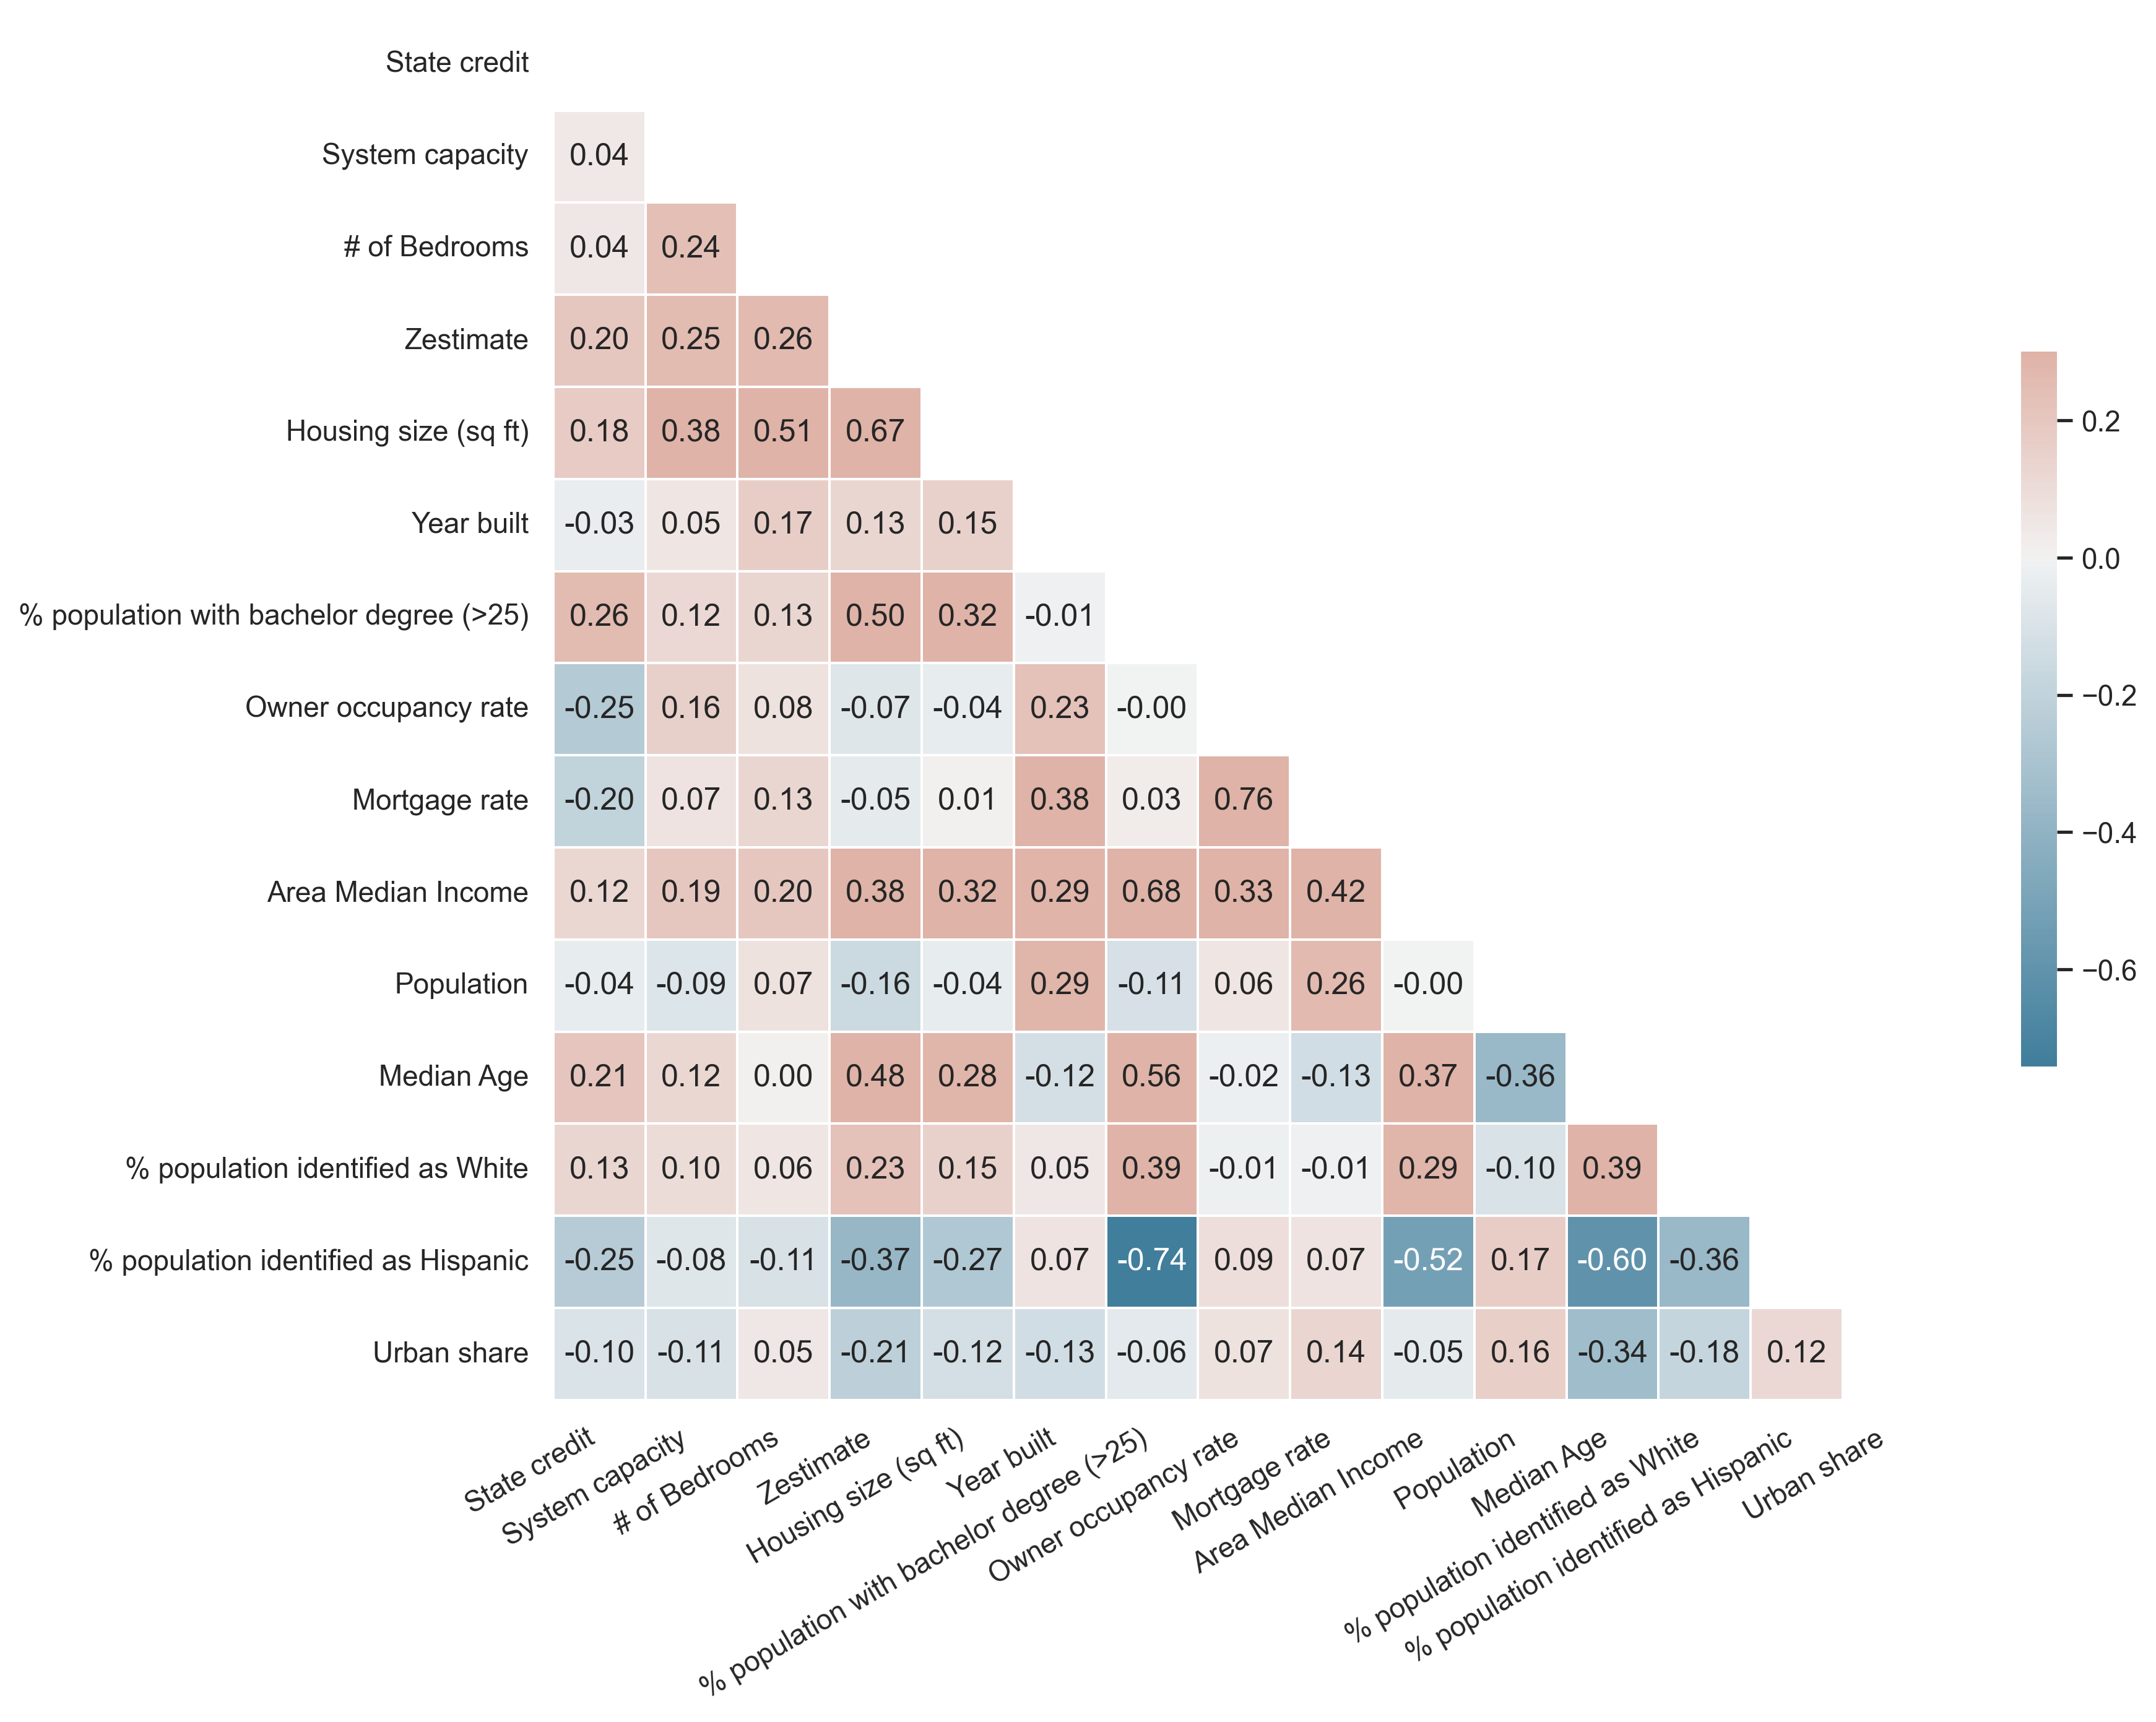
\includegraphics[width=1\textwidth]{figures/corr_matrix.png}
    \caption{Correlation matrix between regression variables}
    \label{fig:corr_matrix}
\end{figure}

\begin{figure}[H]
    \centering
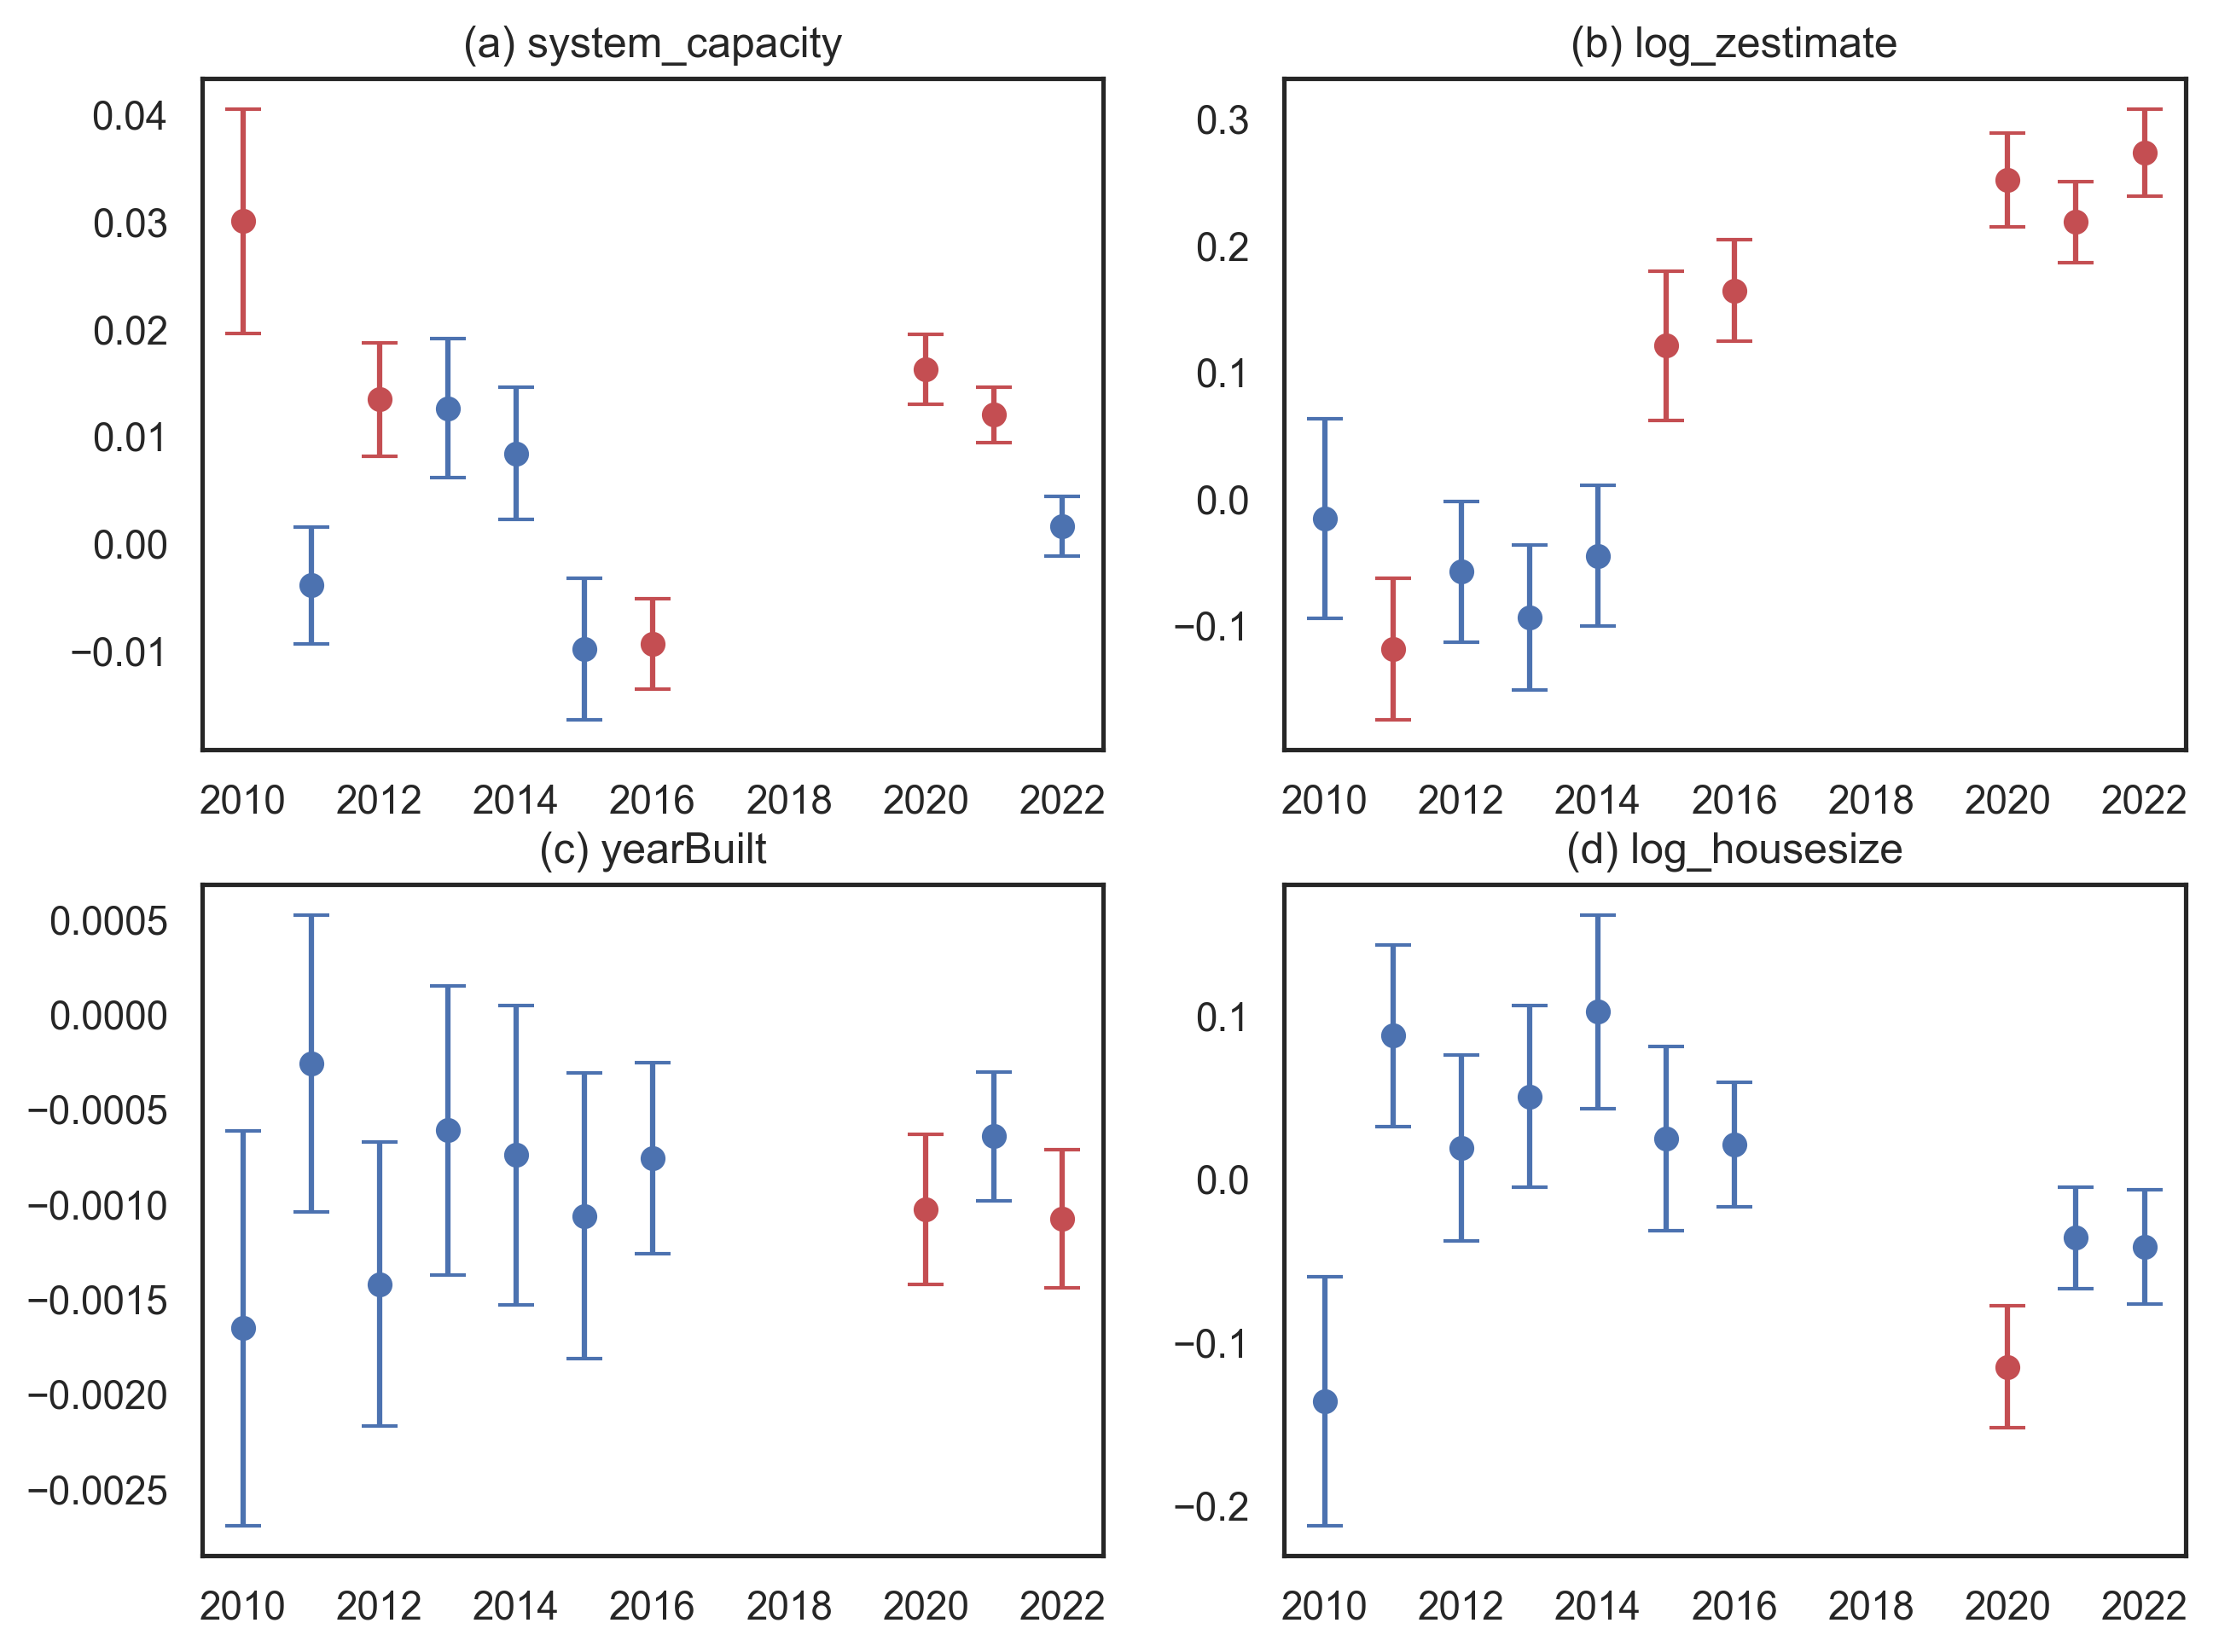
\includegraphics[width=0.9\textwidth]{figures/key_coefficient_trend.png}
    \caption{Coefficient trend by year for key explanatory variables}
    \label{fig:coefficient_trend}
\end{figure}




%%%%%%%%%%%%%%%%%%%%%%%%%%%%%%%%%%%
\newpage

\printbibliography

\end{document}
